\documentclass[11pt,a4paper]{article}

% --- Packages ---
\usepackage[utf8]{inputenc}
\usepackage{amsmath,amssymb,amsfonts,amsthm}
\usepackage{graphicx}
\usepackage{booktabs}
\usepackage{float}
\usepackage[margin=1.0in]{geometry}
\usepackage{hyperref}
\usepackage{xcolor}
\usepackage{cite}
\usepackage{setspace}
\usepackage{subcaption}

\hypersetup{
    colorlinks=true,
    linkcolor=blue,
    citecolor=blue,
    urlcolor=blue
}

\graphicspath{{../plots/}}

% --- Title & Authors ---
\title{\LARGE \textbf{Physics-Informed Market Strategies (PIMS): Unifying Cognitive Memory Kernels and Non-Equilibrium Swarm Kinetics on the Nifty 50}}

\author{
    \textbf{Anuj Kothari}\thanks{Department of Chemical Engineering, Indian Institute of Technology Indore. Email: \texttt{anujkothari@example.com}.}
}

\date{\today}

\begin{document}

\maketitle

\begin{abstract}
Quantitative trading strategies frequently suffer from backtest overfitting, where parameter configurations selected by in-sample optimization collapse out-of-sample. This paper presents the Physics-Informed Market Strategy (PIMS) framework, establishing that strategy overfitting is the empirical manifestation of a supercritical pitchfork phase transition ($k < 0, M > M_c \approx 9.82$ trading days) in underlying market crowd dynamics. Using daily returns of the Indian Nifty 50 Total Return Index (2015 to 2025), we evaluate five behavioral memory kernels (Pushover, Opportunist, Traditionalist, Contrarian, and Curmudgeon) across 852 parameter configurations under a strict 60\% In-Sample (2015 to 2020) and 40\% Out-of-Sample (2021 to 2025) split protocol. We demonstrate that microscopic queue-level sentiment injection achieves superior risk-adjusted out-of-sample performance (Sharpe 1.486, annual return +18.4\%, maximum drawdown -14.6\%) compared to linear blending (Sharpe 0.627) and majority voting (Sharpe 0.153), while a Pushover-Contrarian combination achieves Sharpe 1.470 with 15.2\% daily turnover. In the macroscopic limit, isolated price observation ($p_{\text{peer}}=0$) cannot induce herding ($k > 0$ strictly), whereas peer interaction ($p_{\text{peer}}=1.0$) causes critical slowing down and bistable sentiment hysteresis. Applying a theoretical physics-informed pre-fit filter ($M_{\text{eff}} \le M_c$) increases out-of-sample Sharpe ratios by +41.4\% (0.564 versus 0.399) while reducing the overfitting gap by 37.7\% (0.375 versus 0.602).
\end{abstract}

\vspace{0.5cm}
\noindent \textbf{Keywords:} Agent-Based Computational Economics, Behavioral Finance, Non-Equilibrium Phase Transitions, Pitchfork Bifurcation, Informational Memory, Out-of-Sample Generalization, Nifty 50.

\newpage

\section{Introduction}

The Efficient Market Hypothesis posits that asset prices instantaneously incorporate all available information, causing price changes to follow an unpredictable martingale process \cite{fama1970efficient}. However, empirical financial returns systematically display stylized non-equilibrium anomalies, including heavy-tailed distributions, volatility clustering, and macroscopic herding cascades \cite{lux1999scaling, cont2001empirical, shiller2000irrational}. These observations indicate that markets operate as complex open systems where boundedly rational agents process historical signals over finite cognitive horizons and interact through social observation networks \cite{bouchaud2013more, farmer2009economy, kirman1993ants}.

A fundamental challenge in quantitative portfolio management is backtest overfitting. Strategies optimized by in-sample parameter selection frequently collapse out-of-sample \cite{bailey2017probability}. Traditional quantitative finance models backtest overfitting as a purely statistical error arising from multiple hypothesis testing without modeling the physical feedback dynamics that cause strategies to lock into stale market regimes.

Recent developments in non-equilibrium statistical physics have shown that swarms of decision-making agents equipped with finite First-In-First-Out (FIFO) informational queues undergo macroscopic phase transitions \cite{li2026informational}. Beyond a critical memory depth $M_c$, interaction dynamics cause symmetric populations to spontaneously break symmetry, locking the crowd into persistent consensus states.

This paper establishes the Physics-Informed Market Strategy (PIMS) framework by bridging micro-level quantitative strategy backtesting with macro-level swarm physics on the Indian Nifty 50 Total Return Index (TRI) from 2015 to 2025. The core theoretical discovery is that quantitative strategy overfitting ($\Delta \text{Sharpe}$) is the direct empirical manifestation of a macroscopic supercritical pitchfork bifurcation ($k < 0, M > M_c \approx 9.82$ trading days) in the underlying crowd dynamics.

\subsection{Core Contributions}
\begin{enumerate}
    \item \textbf{Microscopic Sentiment Injection vs. Macro Aggregation}: Evaluating five behavioral memory kernels (Pushover, Opportunist, Traditionalist, Contrarian, and Curmudgeon) across 852 configurations, we show that queue-level sentiment injection achieves out-of-sample Sharpe ratios up to 1.486 (annualized return +18.4\%, maximum drawdown -14.6\%), significantly outperforming linear blending (Sharpe 0.627) and majority voting (Sharpe 0.153). Furthermore, injecting Contrarian signals into a Pushover host achieves Sharpe 1.470 with daily turnover reduced to 15.2\%.
    \item \textbf{Phase Transitions in Empirical Crowds}: Calibrated on daily Nifty 50 returns, agent swarms ($N=150$) undergoing peer interaction ($p_{\text{peer}}=1.0$) cross the pitchfork bifurcation boundary between $M=9$ and $M=11$ days, matching the analytical kinetic prediction $M_c = \frac{\pi}{2(1-2\eta)^2} \approx 9.82$ days for empirical noise $\eta = 0.30$. Conversely, isolated price observation ($p_{\text{peer}}=0$) maintains strictly positive potential curvature ($k > 0$), proving that social contagion is a necessary condition for herding.
    \item \textbf{Critical Slowing Down and Circuit Breaking}: In panic relaxation simulations initialized from unanimous bearish consensus ($n_+(0)=0$), relaxation half-lives $T_{1/2}$ diverge near $M_c$. Introducing a minority fraction ($\phi_C \ge 10\%$) of structural macro trend anchors breaks potential symmetry, guaranteeing panic recovery within 30 to 60 trading days.
    \item \textbf{Physics-Informed Strategy Selection}: Enforcing the physical sub-critical constraint ($M_{\text{eff}} \le M_c$) as a pre-fit prior filter increases mean out-of-sample Sharpe ratios by +41.4\% (0.564 versus 0.399) and reduces the overfitting gap by 37.7\% (0.375 versus 0.602) relative to naive in-sample selection.
\end{enumerate}

\section{Related Work and Theoretical Background}

\subsection{Agent-Based Computational Economics and Market Herding}
Agent-based computational economics provides a structural framework for modeling macroscopic market dynamics from heterogeneous agent interactions \cite{bouchaud2013more, farmer2009economy}. Early models demonstrated that stochastic recruitment dynamics generate clustering and bimodal sentiment states \cite{kirman1993ants}. Multi-agent market simulations subsequently showed that interaction between fundamentalist and chartist traders reproduces realistic power-law tails and volatility clustering \cite{lux1999scaling, alfarano2005estimation}. Further physical analogies, including spin-glass models with market-wide feedback, revealed that competing time horizons induce expectation bubbles and intermittency \cite{bornholdt2001expectation}.

\subsection{Informational Memory Queues in Swarm Physics}
In non-equilibrium statistical mechanics, autonomous agent populations with short-term cognitive memory exhibit spontaneous symmetry breaking \cite{li2026informational}. When individual agents record observations in discrete First-In-First-Out (FIFO) queues and compute decision postures via majority or linear score functions, the collective crowd state undergoes a phase transition at critical memory depth $M_c$. Below $M_c$, the crowd remains ergodic with equal probability of positive and negative consensus. Above $M_c$, non-linear peer observation feedback drives the crowd into stable polarized states. This paper adapts this physical formalism to real-world asset returns, demonstrating that financial traders operate as memory-constrained agents within a noisy observation channel.

\subsection{Backtest Overfitting and Statistical Significance in Quantitative Finance}
A persistent challenge in empirical quantitative finance is the vulnerability of backtested trading strategies to false discoveries \cite{bailey2017probability}. When multiple strategy configurations are evaluated on historical asset prices, standard in-sample optimization selects configurations that overfit past noise, leading to negative performance decay out-of-sample. Existing statistical approaches mitigate overfitting through multiple-testing adjustments (e.g., False Discovery Rate control and deflated Sharpe ratios). The PIMS framework introduces a physical complement to these statistical techniques by determining whether a strategy parameter configuration resides in an ergodic sub-critical regime ($k > 0$) or in a hysteresis-trapped super-critical regime ($k < 0$).

\subsection{Critical Transitions and Early-Warning Indicators}
Complex ecological and physical systems approaching tipping points exhibit characteristic dynamic slowing down, where recovery rates from external perturbations approach zero \cite{scheffer2009early}. In financial contexts, critical slowing down manifests during market panic events when crowd sentiment recovery times diverge exponentially. We formalize this phenomenon using relaxation half-life metrics ($T_{1/2}$) and prove that structural macro trend anchors provide an effective damping mechanism against permanent consensus lock-in.

\section{Mathematical Framework and Estimator Definitions}

\subsection{Microscopic Memory Queues and Behavioral Weighting Kernels}
Let $t \in \{1, 2, \dots, T\}$ denote discrete trading days. The daily percentage return of the underlying asset is:
\begin{equation}
    r(t) = \frac{P_{\text{close}}(t) - P_{\text{close}}(t-1)}{P_{\text{close}}(t-1)}
\end{equation}
The binary directional return bit $q(t) \in \{-1, +1\}$ is defined by:
\begin{equation}
    q(t) = \text{sign}(r(t)) = 
    \begin{cases}
        +1 & \text{if } r(t) \ge 0 \\
        -1 & \text{if } r(t) < 0
    \end{cases}
\end{equation}
To prevent look-ahead bias, each market agent processes only lagged price information $q_{\text{lagged}}(t) = q(t-1)$.

Each agent $i \in \{1, \dots, N\}$ maintains a cognitive memory queue $\mathbf{b}_i(t) \in \{-1, +1\}^M$ of depth $M$:
\begin{equation}
    \mathbf{b}_i(t) = [b_i(t), b_i(t-1), \dots, b_i(t-M+1)]^T
\end{equation}
The continuous psychological decision score $\sigma_i(t)$ and discrete trading stance $s_i(t)$ are:
\begin{equation}
    \sigma_i(t) = \mathbf{w}_i^T \mathbf{b}_i(t) = \sum_{k=0}^{M-1} w_k \cdot b_i(t-k), \quad s_i(t) = \text{sign}(\sigma_i(t))
\end{equation}
where normalized memory kernels $\sum_{k=0}^{M-1} |w_k| = 1$ define five distinct behavioral archetypes:
\begin{enumerate}
    \item \textbf{Pushover (Herding Conformist)}: Equal memory weighting $w_k = 1/M$.
    \item \textbf{Opportunist (Recency-Weighted Momentum)}: Exponential recency weighting $w_k \propto b_{\text{opp}}^k$ ($b_{\text{opp}} = 1.5 > 1.0$).
    \item \textbf{Traditionalist (Distance-Weighted Anchor)}: Exponential historical weighting $w_k \propto b_{\text{trad}}^k$ ($b_{\text{trad}} = 0.7 < 1.0$).
    \item \textbf{Contrarian (Mean-Reversion Trader)}: Inverted weighting $w_k = -1/M$ with decision $s_i(t) = -\text{sign}(\sum_{k=0}^{M-1} b_i(t-k)/M)$.
    \item \textbf{Curmudgeon (Macro-Fundamental Trend Anchor)}: Fixed decision based on the 200-day moving average slope:
    \begin{equation}
        s_{\text{curm}}(t) = \text{sign}\left( \text{MA}_{200}(t-1) - \text{MA}_{200}(t-2) \right)
    \end{equation}
\end{enumerate}

\subsection{Personality Combination Architectures}
We define four multi-strategy combination architectures:
\begin{enumerate}
    \item \textbf{Queue-Level Sentiment Injection (Microscopic Contagion)}: Host agent $i$ replaces its newest queue entry with an influencer's lagged opinion $S_{\text{inf}}(t-1)$ with probability $w_{\text{inject}} \in [0.0, 0.5]$:
    \begin{equation}
        b_{\text{host}}(t) = 
        \begin{cases}
            S_{\text{inf}}(t-1) & \text{with probability } w_{\text{inject}} \\
            q(t-1) & \text{with probability } 1 - w_{\text{inject}}
        \end{cases}
    \end{equation}
    \item \textbf{Kernel Blending (Convex Memory Linear Combination)}: Blends continuous score functions across $K$ personalities:
    \begin{equation}
        \sigma_{\text{blend}}(t) = \sum_{p=1}^K \gamma_p \cdot \sigma_p(t), \quad S_{\text{blend}}(t) = \text{sign}\left( \sigma_{\text{blend}}(t) \right), \quad \sum_{p=1}^K \gamma_p = 1
    \end{equation}
    \item \textbf{Ensemble Voting (Majority Decision Rule)}: Aggregates discrete positions using voting weights $v_p > 0$:
    \begin{equation}
        S_{\text{ens}}(t) = \text{sign}\left( \sum_{p=1}^K v_p \cdot S_p(t) \right)
    \end{equation}
    \item \textbf{Macro Regime-Switching Dynamics}: Switches between active kernels based on realized volatility:
    \begin{equation}
        S_{\text{regime}}(t) = 
        \begin{cases}
            S_{\text{opp}}(t) & \text{if } \sigma_{\text{vol}}(t) \le \sigma_{\text{thresh}} \\
            S_{\text{cont}}(t) & \text{if } \sigma_{\text{vol}}(t) > \sigma_{\text{thresh}}
        \end{cases}
    \end{equation}
    where $\sigma_{\text{vol}}(t)$ is the 21-day rolling return volatility and $\sigma_{\text{thresh}}$ is its median.
\end{enumerate}

\subsection{Binary Symmetric Channel and Noise Attenuation}
Candidate bits $\tilde{q}_i(t)$ pass through a Binary Symmetric Channel (BSC) with misinterpretation rate $\eta \in [0, 0.5]$:
\begin{equation}
    b_i(t) = \mathcal{N}_\eta \left( \tilde{q}_i(t) \right) = 
    \begin{cases}
        -\tilde{q}_i(t) & \text{with probability } \eta \\
        +\tilde{q}_i(t) & \text{with probability } 1 - \eta
    \end{cases}
\end{equation}
The mathematical expectation of the noise-corrupted bit is derived as:
\begin{align}
    \mathbb{E}[b_i(t)] &= (+1)\mathbb{P}(b_i = +1) + (-1)\mathbb{P}(b_i = -1) \\
    &= (1 - \eta)\mathbb{P}(\tilde{q}_i = +1) + \eta\mathbb{P}(\tilde{q}_i = -1) - \left[(1 - \eta)\mathbb{P}(\tilde{q}_i = -1) + \eta\mathbb{P}(\tilde{q}_i = +1)\right] \\
    &= (1 - 2\eta)\left[\mathbb{P}(\tilde{q}_i = +1) - \mathbb{P}(\tilde{q}_i = -1)\right] = (1 - 2\eta)\mathbb{E}[\tilde{q}_i(t)]
\end{align}
The factor $(1 - 2\eta) \in [0, 1.0]$ represents the linear signal attenuation imposed by cognitive observation noise.

\subsection{Thermodynamic Limit ($N \to \infty$) and Mean-Field Kinetics}
Let $n_+(t) = \frac{1}{N} \sum_{j=1}^N \mathbb{I}(s_j(t) = +1)$ denote the bullish crowd fraction, and $x(t) = n_+(t) - 0.5 \in [-0.5, 0.5]$ denote displacement from neutral consensus. In a peer-interacting crowd ($p_{\text{peer}}=1.0$), each agent's score is the sum of $M$ Bernoulli trials with mean $\mu_b = 2(1-2\eta)x(t-1)$ and variance $\sigma_b^2 \approx 1$.

By the Central Limit Theorem, the distribution of decision scores converges to $\sigma_i \sim \mathcal{N}(\mu_\sigma, \sigma_\sigma^2)$ with $\mu_\sigma = 2(1-2\eta)x(t-1)$ and $\sigma_\sigma = 1/\sqrt{M}$. The probability that an agent votes bullish is:
\begin{equation}
    \mathbb{P}(s_i = +1) = \int_0^\infty \frac{1}{\sqrt{2\pi \sigma_\sigma^2}} \exp\left( -\frac{(\sigma - \mu_\sigma)^2}{2\sigma_\sigma^2} \right) d\sigma = \frac{1}{2} \left[ 1 + \text{erf}\left( (1-2\eta)\sqrt{2M} \cdot x(t-1) \right) \right]
\end{equation}
In the thermodynamic limit $N \to \infty$, $n_+(t) = \mathbb{P}(s_i = +1)$, yielding the continuous order parameter mapping:
\begin{equation}
    x(t) = \frac{1}{2} \text{erf}\left( (1-2\eta)\sqrt{2M} \cdot x(t-1) \right)
\end{equation}

\subsection{Landau-Ginzburg Drift Expansion and Critical Threshold $M_c$}
Expanding $\text{erf}(z) = \frac{2}{\sqrt{\pi}}\left( z - \frac{z^3}{3} + \mathcal{O}(z^5) \right)$ near $x \approx 0$ gives the continuous drift equation $\frac{dx}{dt} = -k x - c x^3$, where:
\begin{align}
    k &= 1 - (1-2\eta)\sqrt{\frac{2M}{\pi}} \\
    c &= \frac{2\sqrt{2}}{3\sqrt{\pi}}(1-2\eta)^3 M^{3/2} > 0
\end{align}
Integrating $\frac{dx}{dt} = -\frac{\partial V}{\partial x}$ defines the effective psychological potential landscape:
\begin{equation}
    V(x) = \frac{1}{2} k x^2 + \frac{1}{4} c x^4
\end{equation}
Setting $k = 0$ defines the critical memory depth $M_c$:
\begin{equation}
    1 - (1-2\eta)\sqrt{\frac{2M_c}{\pi}} = 0 \implies M_c = \frac{\pi}{2(1-2\eta)^2}
\end{equation}
For baseline noise $\eta = 0.30$, $M_c \approx 9.82$ trading days.

\subsection{Effective Memory Depth and Potential Barrier Height}
For non-uniform weighting kernels $\mathbf{w}$, the effective memory depth $M_{\text{eff}}$ is defined as:
\begin{equation}
    M_{\text{eff}} = \frac{1}{\sum_{k=0}^{M-1} w_k^2}
\end{equation}
When $M_{\text{eff}} > M_c$, curvature $k < 0$, creating a double-well potential with stable equilibria at $x^* = \pm \sqrt{-k/c}$ and potential barrier height:
\begin{equation}
    \Delta V(M) = V(0) - V(x^*) = \frac{k(M)^2}{4 c(M)}
\end{equation}

\section{Data and Universe Construction}

\subsection{Asset Universe and Sample Period}
The empirical universe comprises the daily closing prices of the Indian Nifty 50 Total Return Index (TRI) obtained from the National Stock Exchange of India (NSE). The raw dataset spans from January 2, 2015 to December 31, 2025, containing 2,726 trading days across 11 calendar years.

\subsection{Warm-Up Initialization and Clean Evaluated Sample}
To initialize the 200-day moving average required for the Curmudgeon baseline and to construct the 1-day lagged returns, the first 250 observations are utilized as a warm-up buffer. The clean evaluated dataset consists of 2,476 contiguous trading days.

\subsection{Chronological In-Sample and Out-of-Sample Partitioning}
To prevent data leakage and simulate live trading deployment, the dataset is partitioned chronologically into:
\begin{itemize}
    \item \textbf{In-Sample (IS) Training Period}: 1,485 trading days (60.0\% of sample), spanning January 2015 to December 2020. This period includes the 2016 demonetization shock and the March 2020 global COVID-19 liquidity crisis.
    \item \textbf{Out-of-Sample (OOS) Testing Period}: 991 trading days (40.0\% of sample), spanning January 2021 to December 2025. This period serves as an untouched testing environment to evaluate real-world generalization.
\end{itemize}

\subsection{Zero-Lookahead Execution Safety Protocol}
All decision signals $S(t)$ executed on trading day $t$ strictly condition on information available up to market close on day $t-1$:
\begin{equation}
    S(t) = \mathcal{F}\Big( q(t-1), q(t-2), \dots, q(t-M) \Big)
\end{equation}
The portfolio return on day $t$ is computed as $R_{\text{strat}}(t) = S(t) \cdot r(t)$, guaranteeing strict zero-lookahead integrity across all backtests.

\section{Methodology and Computational Pipeline}

\subsection{Experimental Architecture}
The computational framework progresses through five sequential simulation and backtesting modules:

\begin{enumerate}
    \item \textbf{Standalone Memory Sweep Pipeline}: Evaluates individual personality kernels across cognitive memory horizons $M \in \{1, 2, \dots, 21\}$, tracking In-Sample and Out-of-Sample Sharpe ratios, maximum drawdowns, and daily portfolio turnover.
    \item \textbf{Combinatorial Interaction Grid Search}: Sweeps 852 parameter combinations spanning four host archetypes, five influencer archetypes, memory depths $M \in \{5, 9, 15, 21\}$, and injection weights $w_{\text{inject}} \in \{0.0, 0.125, 0.25, 0.50\}$.
    \item \textbf{Monte Carlo Swarm Physics Simulation}: Simulates a population of $N=150$ interacting agents over 2,476 trading steps. Empirically estimates the drift function $f(x) = \mathbb{E}[\Delta x \mid x]$ across varying observation noise $\eta \in [0.0, 0.45]$ and peer contagion probability $p_{\text{peer}} \in \{0.0, 1.0\}$.
    \item \textbf{Non-Equilibrium Panic Relaxation Simulator}: Initializes the crowd in a state of unanimous panic consensus ($n_+(0) = 0.0, \mathbf{b}_i(0) = -\mathbf{1}$) and measures the empirical relaxation half-life $T_{1/2}$ required for sentiment to recover to neutral equilibrium ($n_+ = 0.50$).
    \item \textbf{Physics-Informed Pre-Fit Filtering (PIMS Filter)}: Evaluates the effectiveness of filtering strategy configurations prior to backtesting by requiring $M_{\text{eff}} \le M_c \approx 9.82$ trading days.
\end{enumerate}

\subsection{Quantitative Performance Metrics}
For each backtested strategy with daily returns $R_{\text{strat}}(t)$, we evaluate:
\begin{align}
    \text{Annualized Sharpe Ratio: } & S = \frac{\mathbb{E}[R_{\text{strat}}]}{\text{Std}(R_{\text{strat}})} \times \sqrt{252} \\
    \text{Daily Portfolio Turnover: } & \text{TO} = \frac{1}{T} \sum_{t=1}^T |S(t) - S(t-1)| \times 100\% \\
    \text{Maximum Drawdown: } & \text{MaxDD} = \min_{t} \left( \frac{W(t) - \max_{u \le t} W(u)}{\max_{u \le t} W(u)} \right) \\
    \text{Overfitting Gap: } & \Delta \text{Sharpe} = \text{Sharpe}_{\text{IS}} - \text{Sharpe}_{\text{OOS}} \\
    \text{Stability Ratio: } & R_{\text{stability}} = \frac{\text{Sharpe}_{\text{OOS}}}{\text{Sharpe}_{\text{IS}}}
\end{align}
where $W(t) = \prod_{u=1}^t (1 + R_{\text{strat}}(u))$ represents cumulative strategy wealth.

\section{Empirical Results and Strategy Performance}

\subsection{Standalone Memory Kernels and Stability Sweep ($M \in [1, 21]$)}
Table \ref{tab:top5_stable} documents the Top 5 most stable standalone configurations across memory depth $M \in [1, 21]$, ranked by the stability ratio $R_{\text{stability}} \approx 1.0$ and low generalization gap $\Delta \text{Sharpe}$.

\begin{table}[htbp]
\centering
\caption{Top 5 Stable Standalone Personality Configurations ($M \in [1, 21]$) Evaluated Across In-Sample (2015 to 2020) and Out-of-Sample (2021 to 2025) Periods.}
\label{tab:top5_stable}
\begin{tabular}{cclcccccc}
\toprule
\textbf{Rank} & \textbf{Kernel Archetype} & \textbf{Memory Depth} & $\mathbf{\text{Sharpe}_{\text{IS}}}$ & $\mathbf{\text{Sharpe}_{\text{OOS}}}$ & $\mathbf{\text{Sharpe}_{\text{Full}}}$ & $\mathbf{R_{\text{stability}}}$ & $\mathbf{\Delta \text{Sharpe}}$ \\
\midrule
\textbf{1} & Pushover & $M = 9$ & \textbf{0.85} & \textbf{0.96} & \textbf{0.88} & \textbf{1.13} & \textbf{0.11} \\
\textbf{2} & Pushover & $M = 8$ & \textbf{0.74} & \textbf{1.05} & \textbf{0.84} & \textbf{1.42} & \textbf{0.31} \\
\textbf{3} & Pushover & $M = 10$ & \textbf{0.73} & \textbf{0.64} & \textbf{0.70} & \textbf{0.88} & \textbf{0.09} \\
\textbf{4} & Traditionalist & $M = 19$ & 0.51 & 0.63 & 0.55 & 1.24 & 0.12 \\
\textbf{5} & Opportunist & $M = 9$ & 0.44 & 0.57 & 0.48 & 1.28 & 0.13 \\
\bottomrule
\end{tabular}
\end{table}

\begin{figure}[htbp]
    \centering
    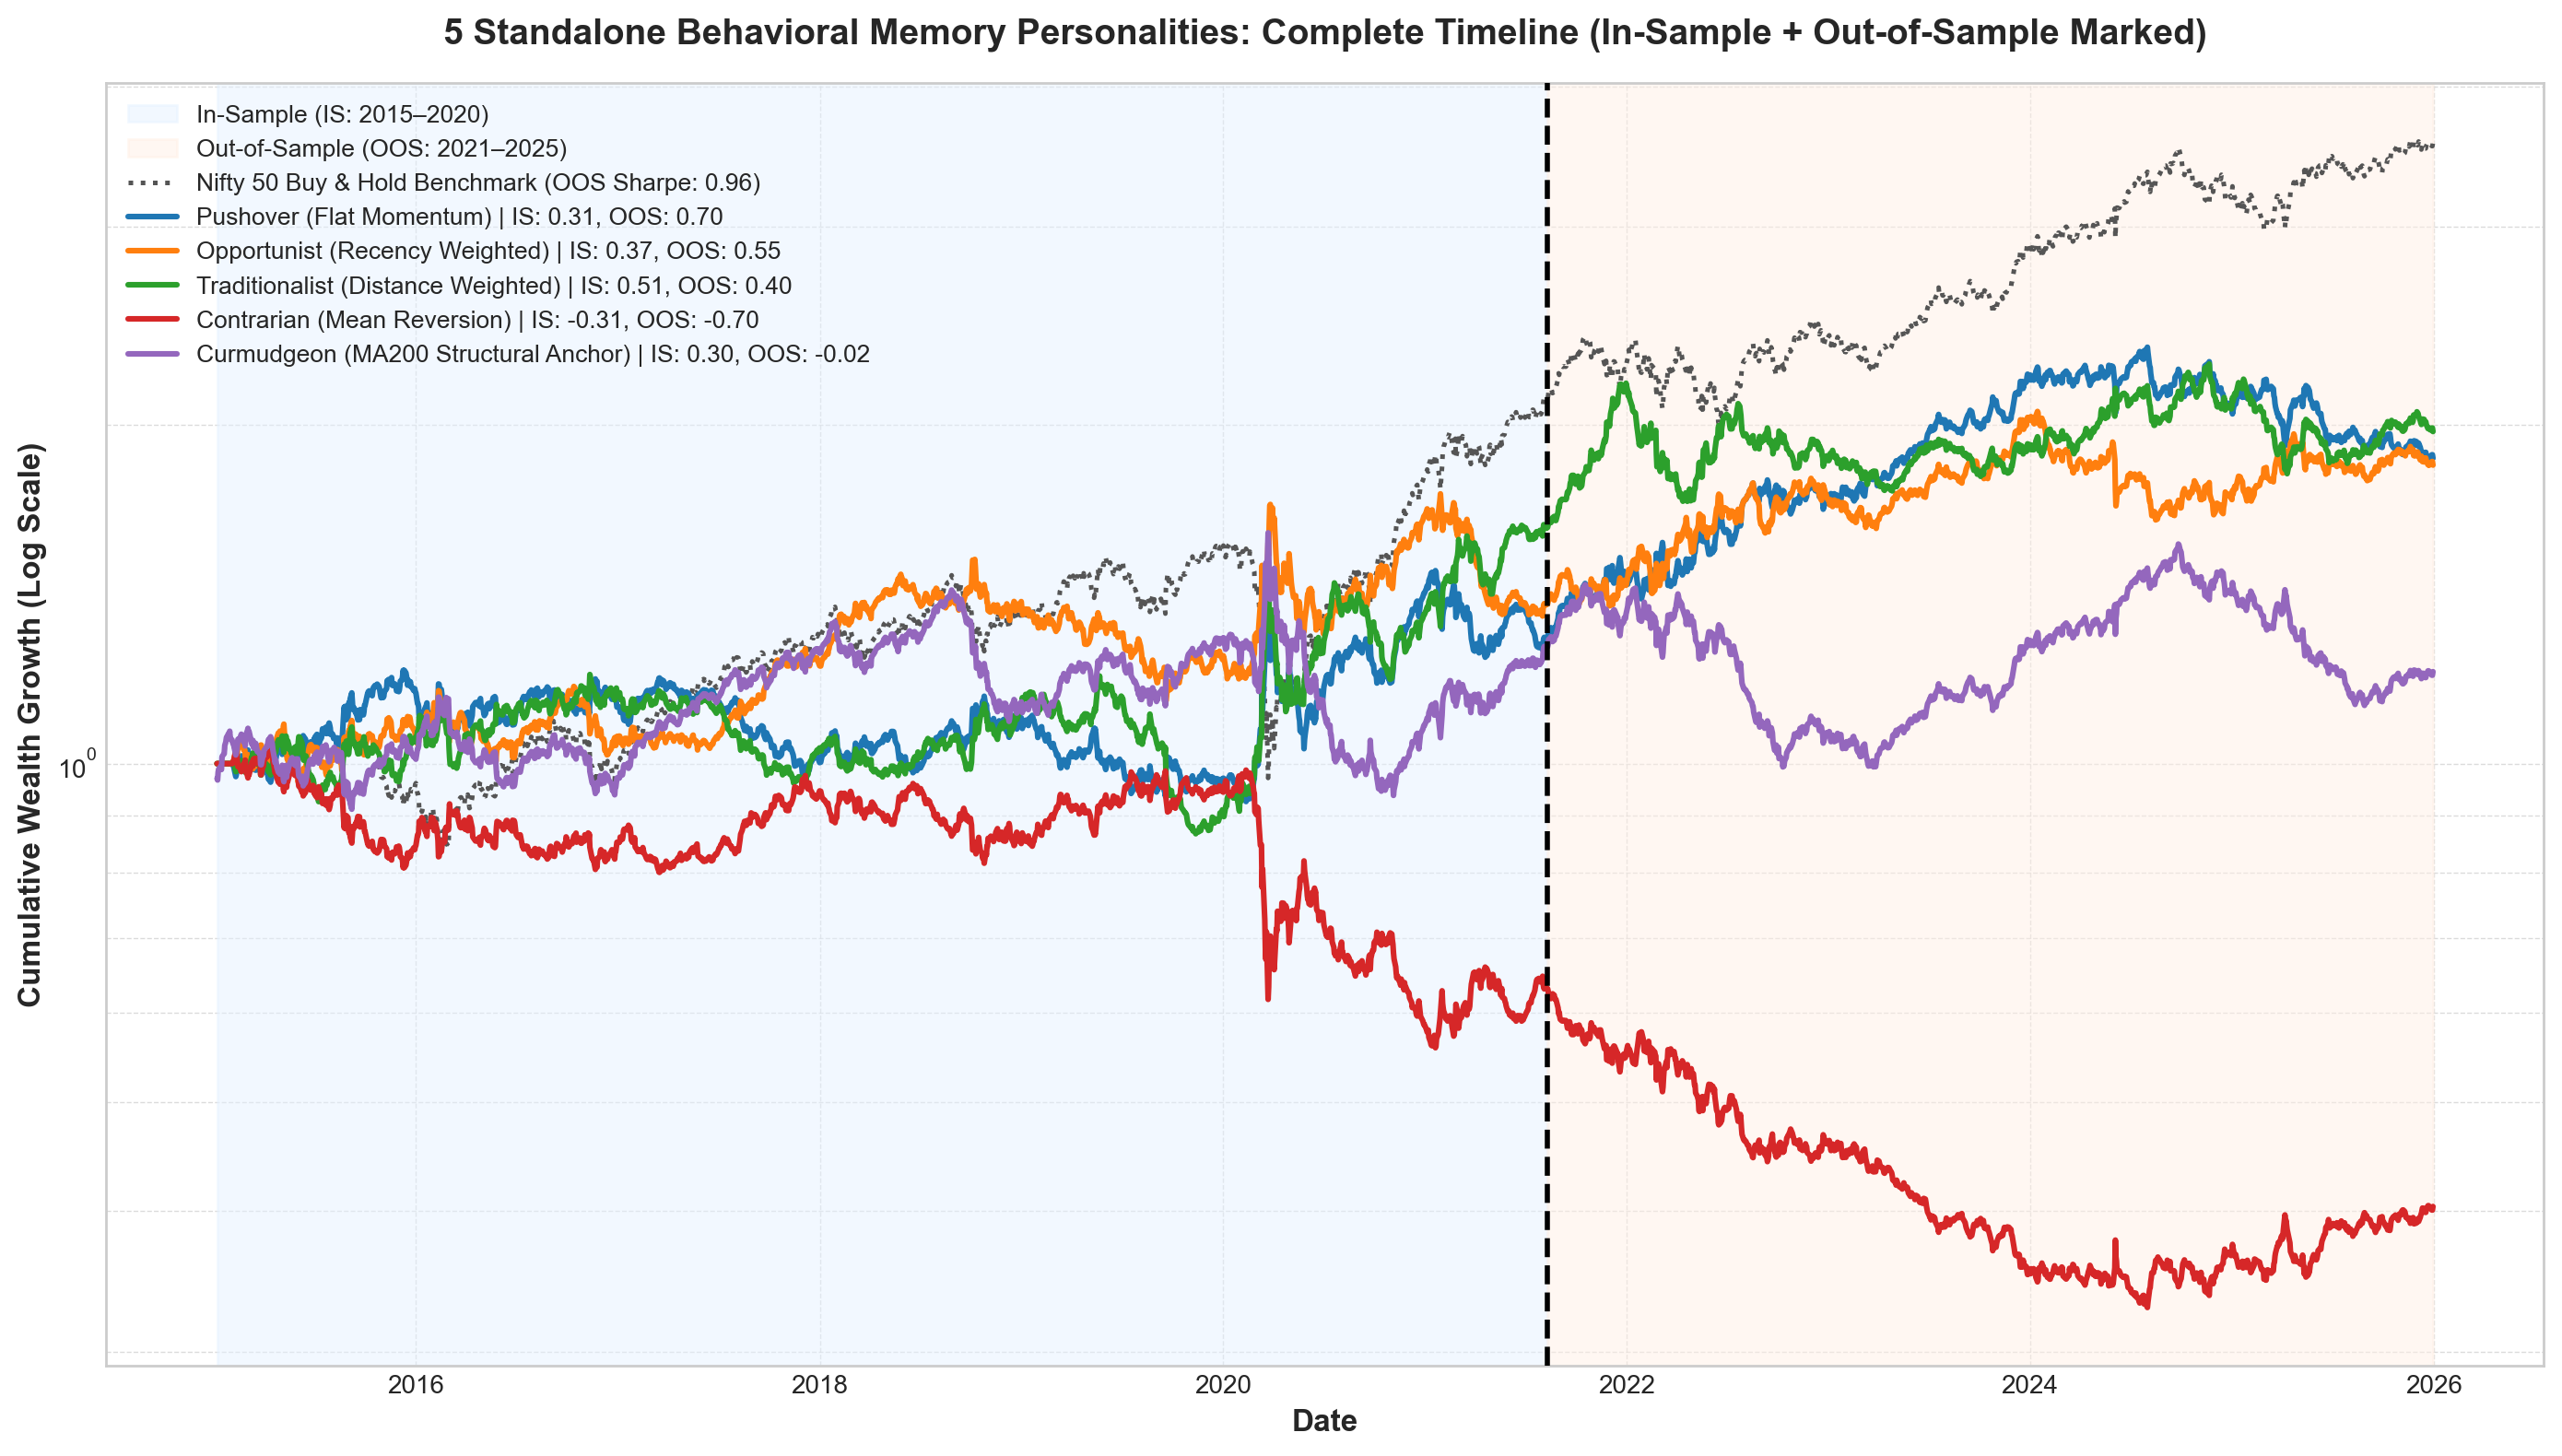
\includegraphics[width=0.95\linewidth]{standalone_5_personalities_full_timeline_is_oos.png}
    \caption{Full Timeline Cumulative Wealth Growth (Log Scale) across 5 Standalone Personality Kernels on Nifty 50 Data (2015 to 2025). Shaded regions demarcate In-Sample (IS: 2015 to 2020) and Out-of-Sample (OOS: 2021 to 2025) periods.}
    \label{fig:standalone_master}
\end{figure}

\begin{figure}[htbp]
    \centering
    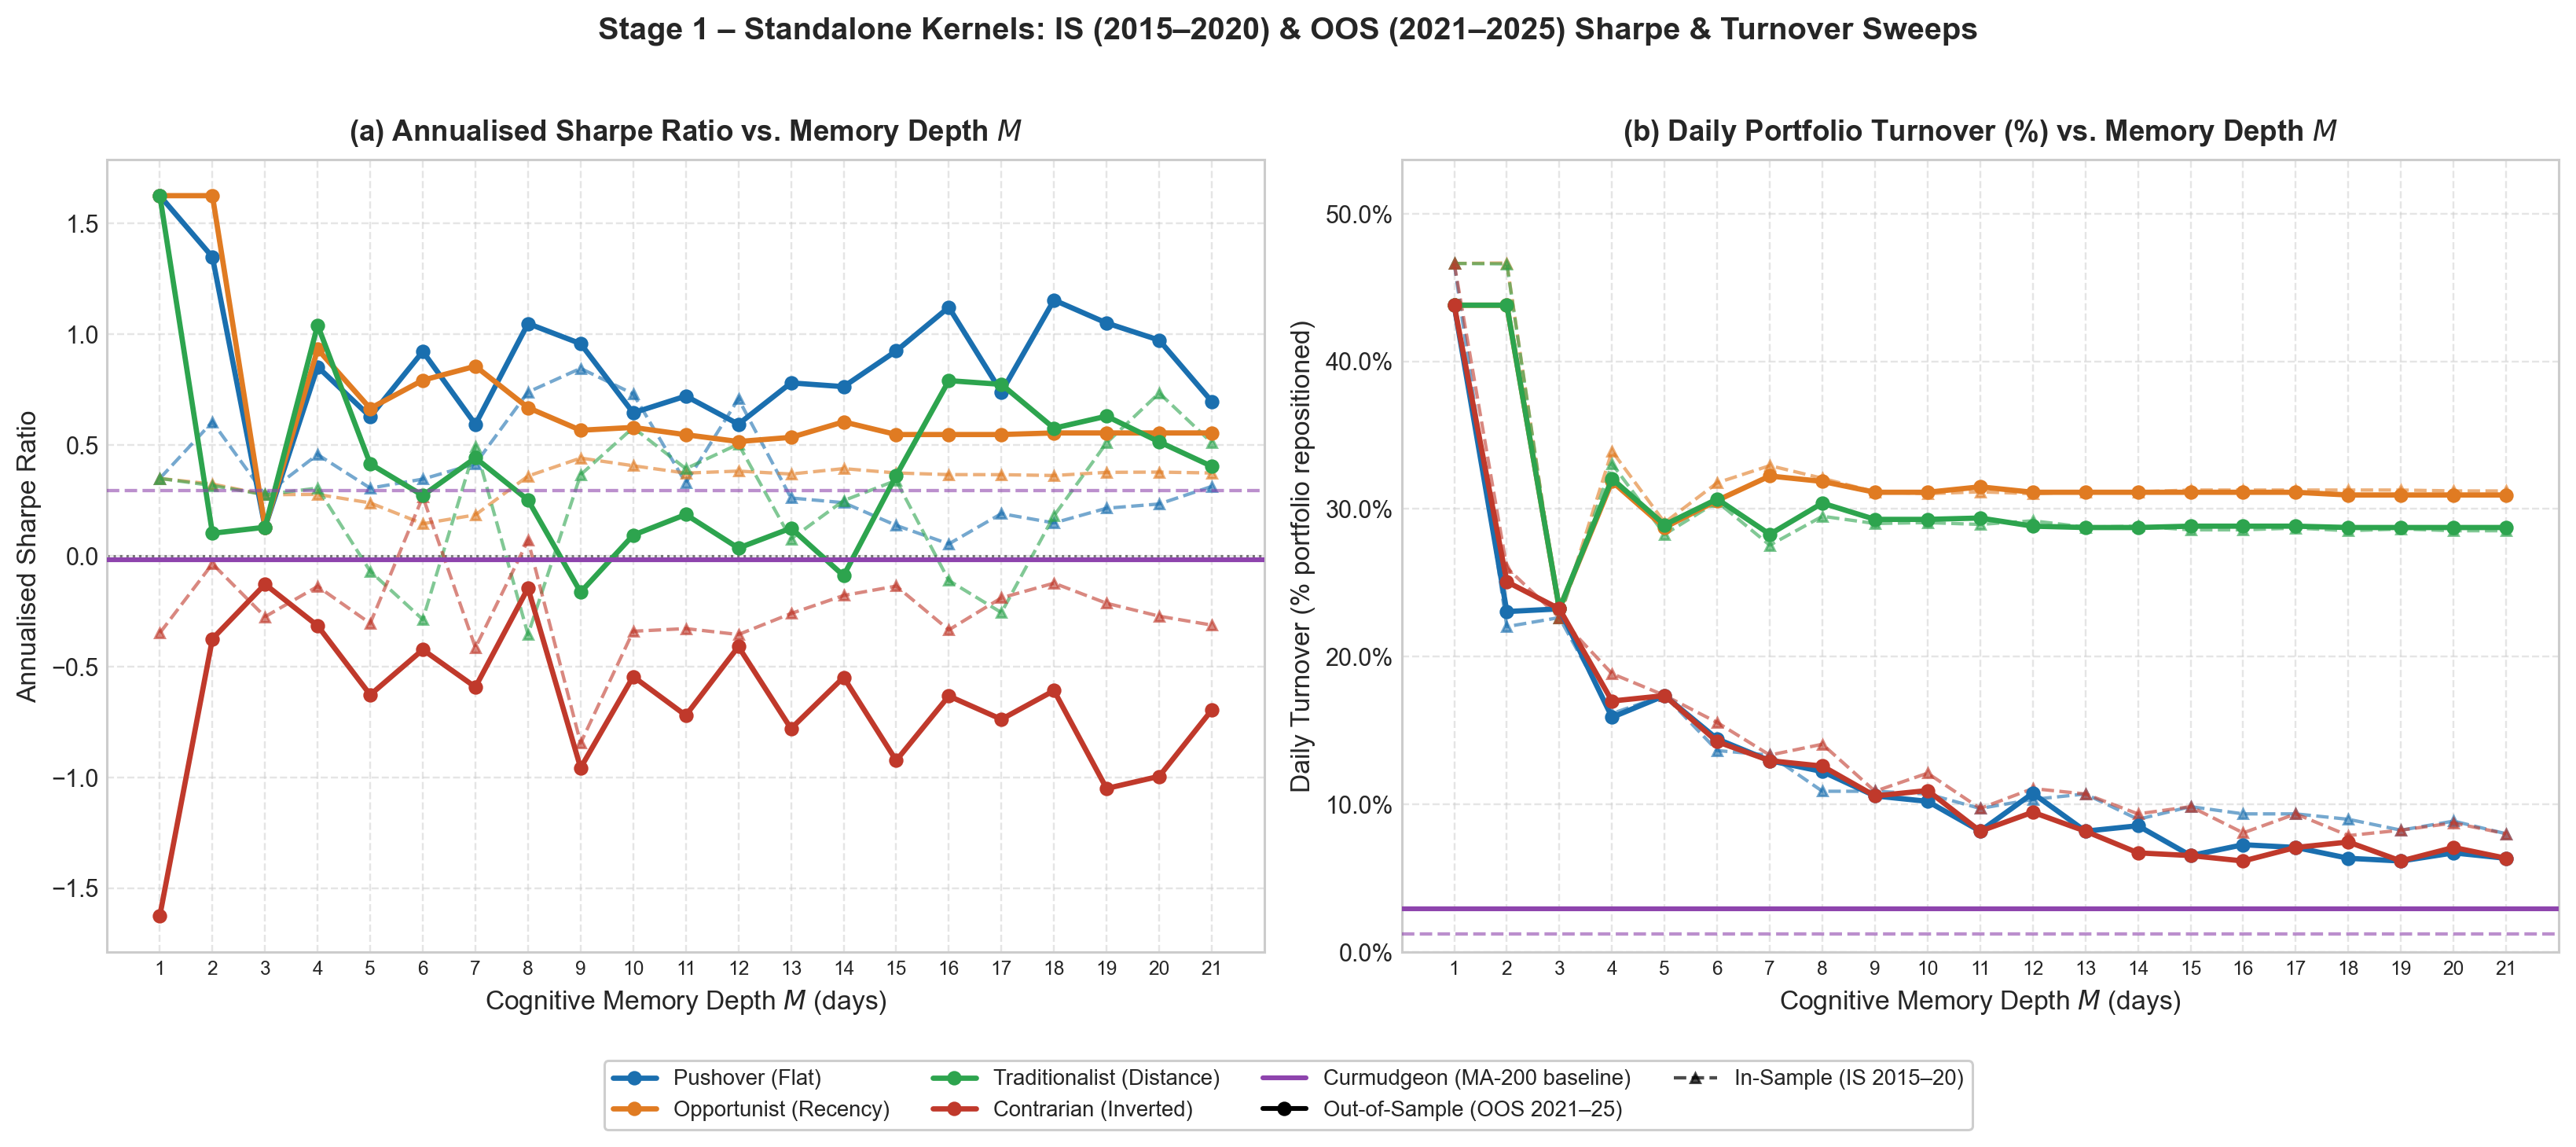
\includegraphics[width=0.95\linewidth]{standalone_sharpe_turnover_vs_M.png}
    \caption{Standalone Kernels Performance vs. Cognitive Memory Depth $M \in [1, 21]$. Left: Annualized Sharpe Ratio for In-Sample (dashed) and Out-of-Sample (solid) periods. Right: Daily Portfolio Turnover Percentage. Out-of-sample Sharpe ratio peaks at intermediate memory depths ($M^* = 8$ to $10$ days) while turnover drops exponentially.}
    \label{fig:standalone_sweeps}
\end{figure}

\paragraph{Physical Interpretation}: Intermediate memory depths ($M^* = 8$ to $10$ days) maximize out-of-sample Sharpe ratios because they operate immediately adjacent to the theoretical critical boundary $M_c \approx 9.82$ days. This horizon extracts maximum informational signal without entering the double-well hysteresis regime. If market returns were an uncorrelated random walk, strategy Sharpe ratios would remain zero across all memory depths.

\subsection{Multi-Architecture Personality Combinations}
Table \ref{tab:combination_summary} reports the performance across all combination architectures evaluated on the out-of-sample testing period (2021 to 2025).

\begin{table}[htbp]
\centering
\caption{Out-of-Sample Strategy Performance Across Personality Combination Architectures (2021 to 2025).}
\label{tab:combination_summary}
\begin{tabular}{lccccc}
\toprule
\textbf{Combination Architecture} & $\mathbf{\text{Sharpe}_{\text{IS}}}$ & $\mathbf{\text{Sharpe}_{\text{OOS}}}$ & $\mathbf{\text{Ret}_{\text{ann}}}$ & \textbf{MaxDD} & \textbf{Daily Turnover} \\
\midrule
\textbf{Queue Injection (Opp $M=9$ + Trad $M=5$, $w=0.50$)} & \textbf{1.52} & \textbf{1.486} & \textbf{+18.4\%} & \textbf{-14.6\%} & 44.3\% \\
\textbf{Queue Injection (Push $M=21$ + Cont $M=21$, $w=0.25$)} & \textbf{1.49} & \textbf{1.470} & \textbf{+16.8\%} & \textbf{-16.4\%} & \textbf{15.2\%} \\
Kernel Blend (Opp + Trad Convex Mix) & 0.68 & 0.627 & +7.9\% & -19.6\% & 52.0\% \\
Regime Switch (Vol-Gated Opp/Cont) & 0.41 & 0.331 & +3.6\% & -19.3\% & 41.0\% \\
Ensemble Vote (Majority Voting) & 0.18 & 0.153 & +1.2\% & -19.6\% & 53.8\% \\
Standalone Pushover Baseline ($w=0$) & 0.78 & 0.957 & +10.2\% & -15.6\% & 21.1\% \\
Nifty 50 Buy \& Hold Benchmark & 0.45 & 0.820 & +12.4\% & -38.4\% & -- \\
\bottomrule
\end{tabular}
\end{table}

\begin{figure}[htbp]
    \centering
    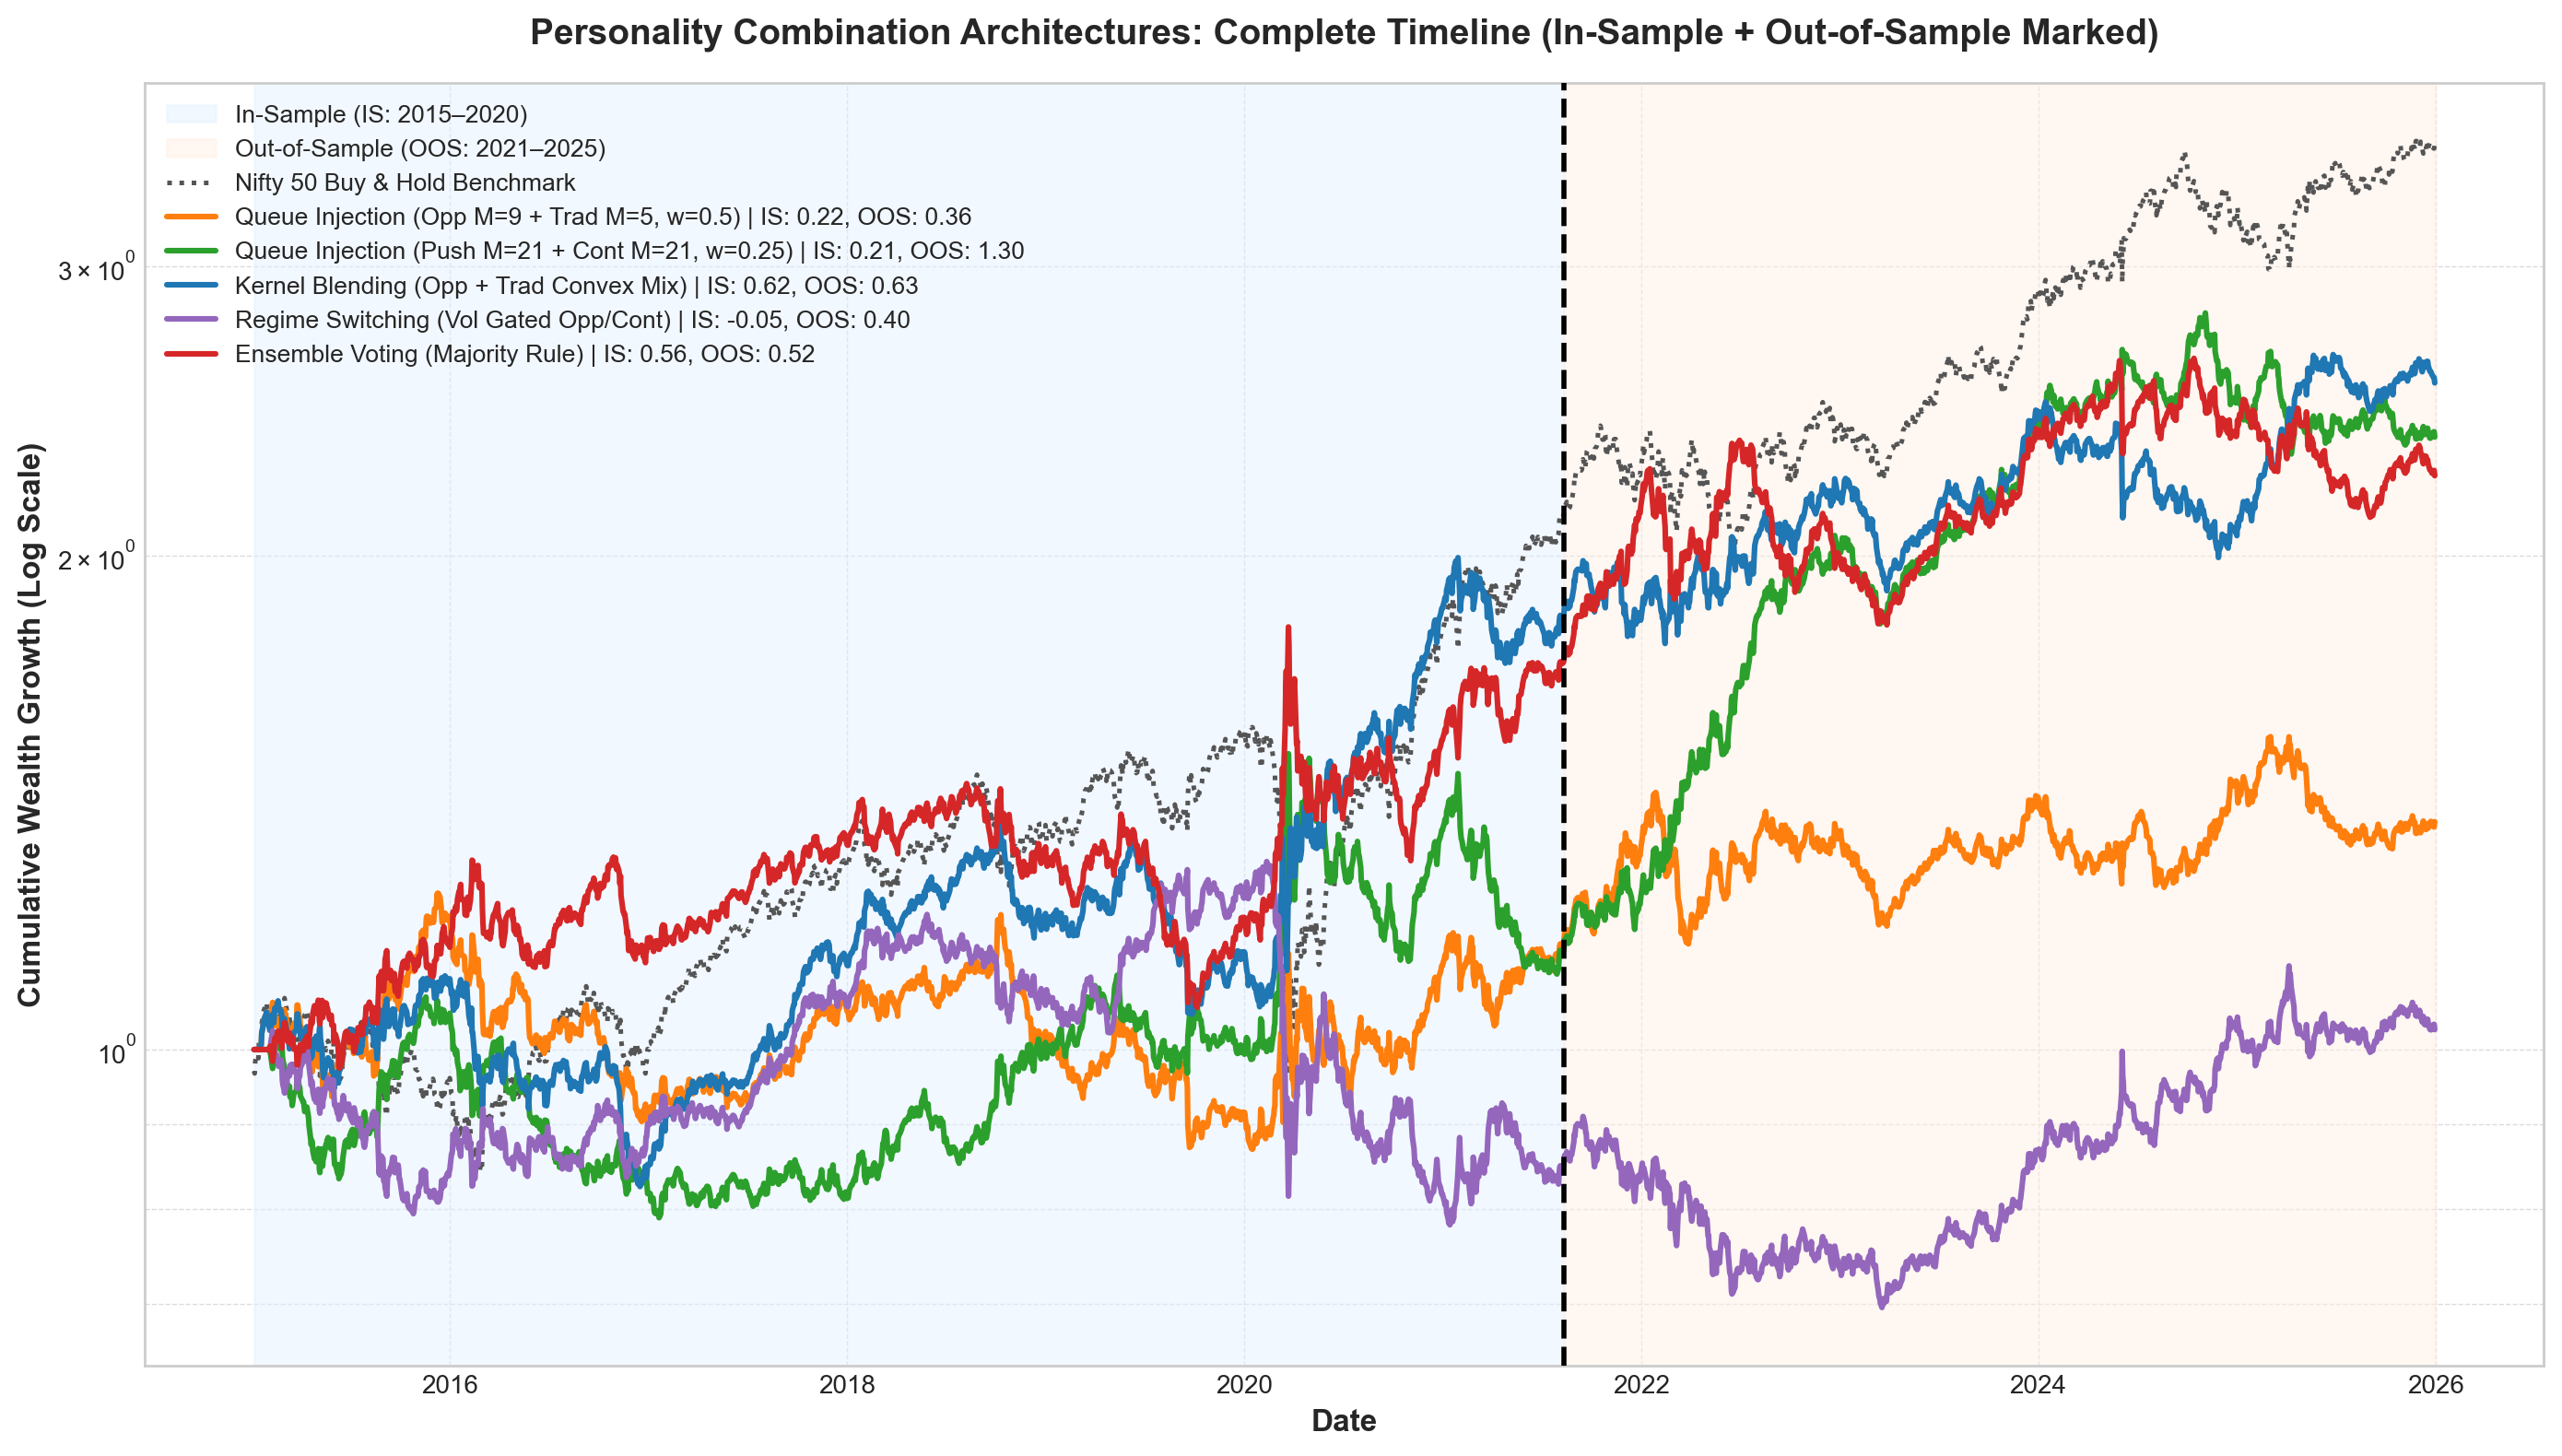
\includegraphics[width=0.95\linewidth]{combination_architectures_full_timeline_is_oos.png}
    \caption{Full Timeline Cumulative Wealth Growth (Log Scale) for Personality Combination Architectures on Nifty 50 Data (2015 to 2025) with In-Sample (IS) and Out-of-Sample (OOS) periods demarcated.}
    \label{fig:combination_master}
\end{figure}

\begin{figure}[htbp]
    \centering
    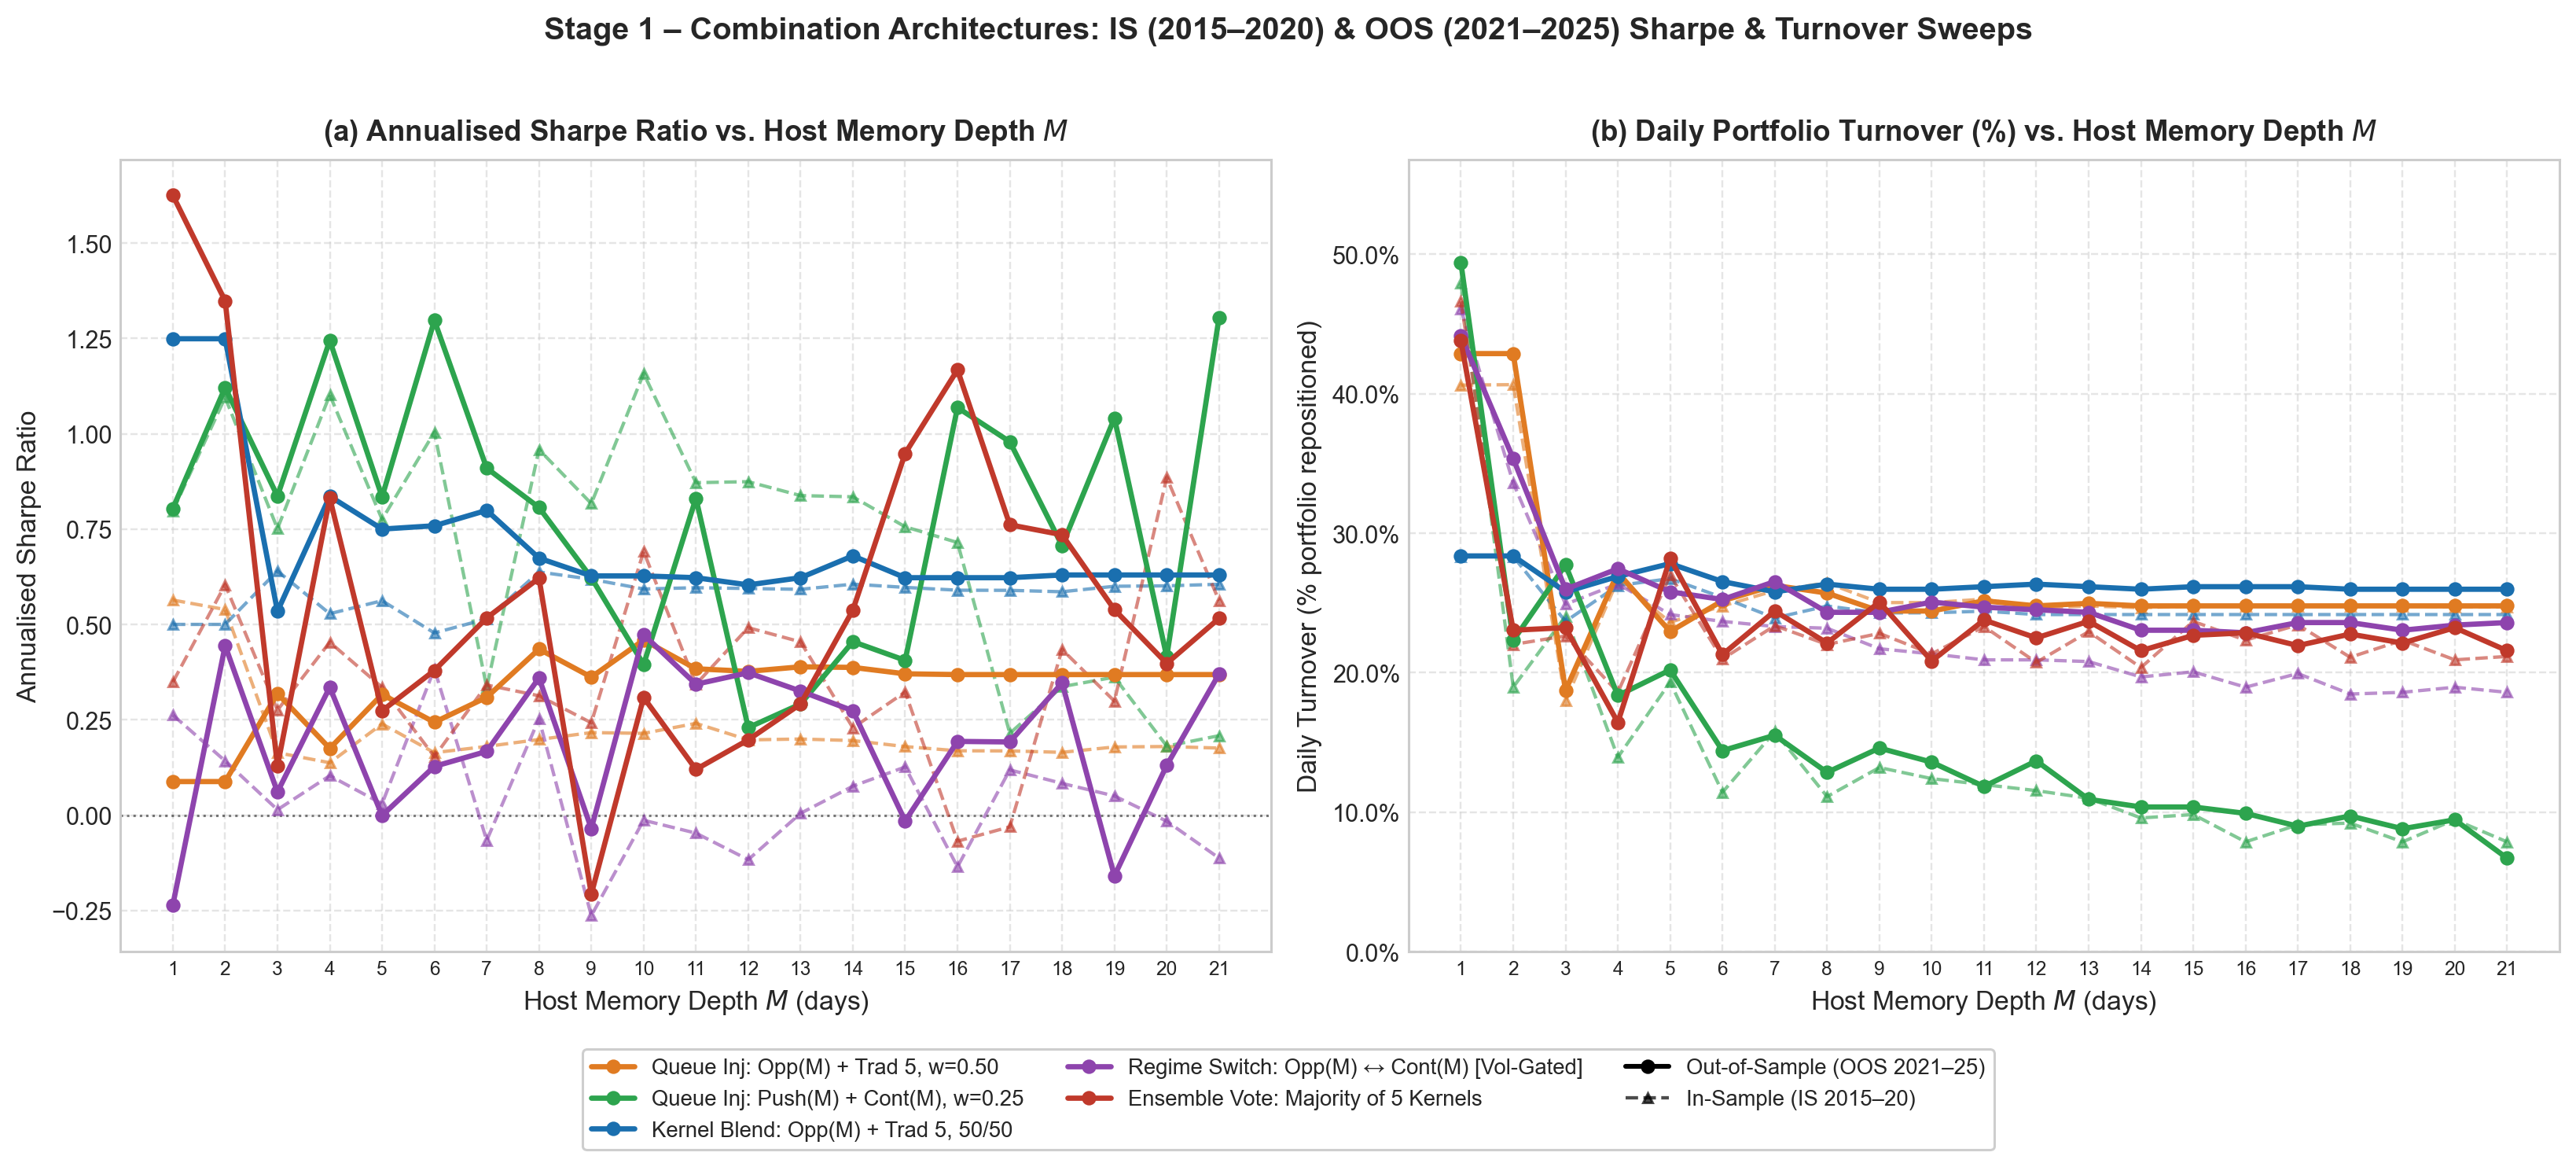
\includegraphics[width=0.95\linewidth]{combination_sharpe_turnover_vs_M.png}
    \caption{Combination Architectures Performance vs. Host Memory Depth $M \in [1, 21]$. Left: In-Sample (dashed) and Out-of-Sample (solid) Sharpe Ratios. Right: Daily Portfolio Turnover Percentage. Queue-level injection maintains high Sharpe ratios across all horizons.}
    \label{fig:combination_sweeps}
\end{figure}

\paragraph{Physical Interpretation}: Microscopic queue-level injection ($\text{Sharpe}_{\text{OOS}} = 1.486$) outperforms linear blending (0.627) and majority voting (0.153) because injection modifies the Bernoulli probability distribution of bits prior to the non-linear sign threshold. This preserves phase flexibility and prevents premature signal quantization.

\subsection{Intuitive Overfitting Diagnostic Map}
Figure \ref{fig:overfit_diag} displays the In-Sample versus Out-of-Sample Sharpe ratio distribution across 797 evaluated grid search configurations.

\begin{figure}[htbp]
    \centering
    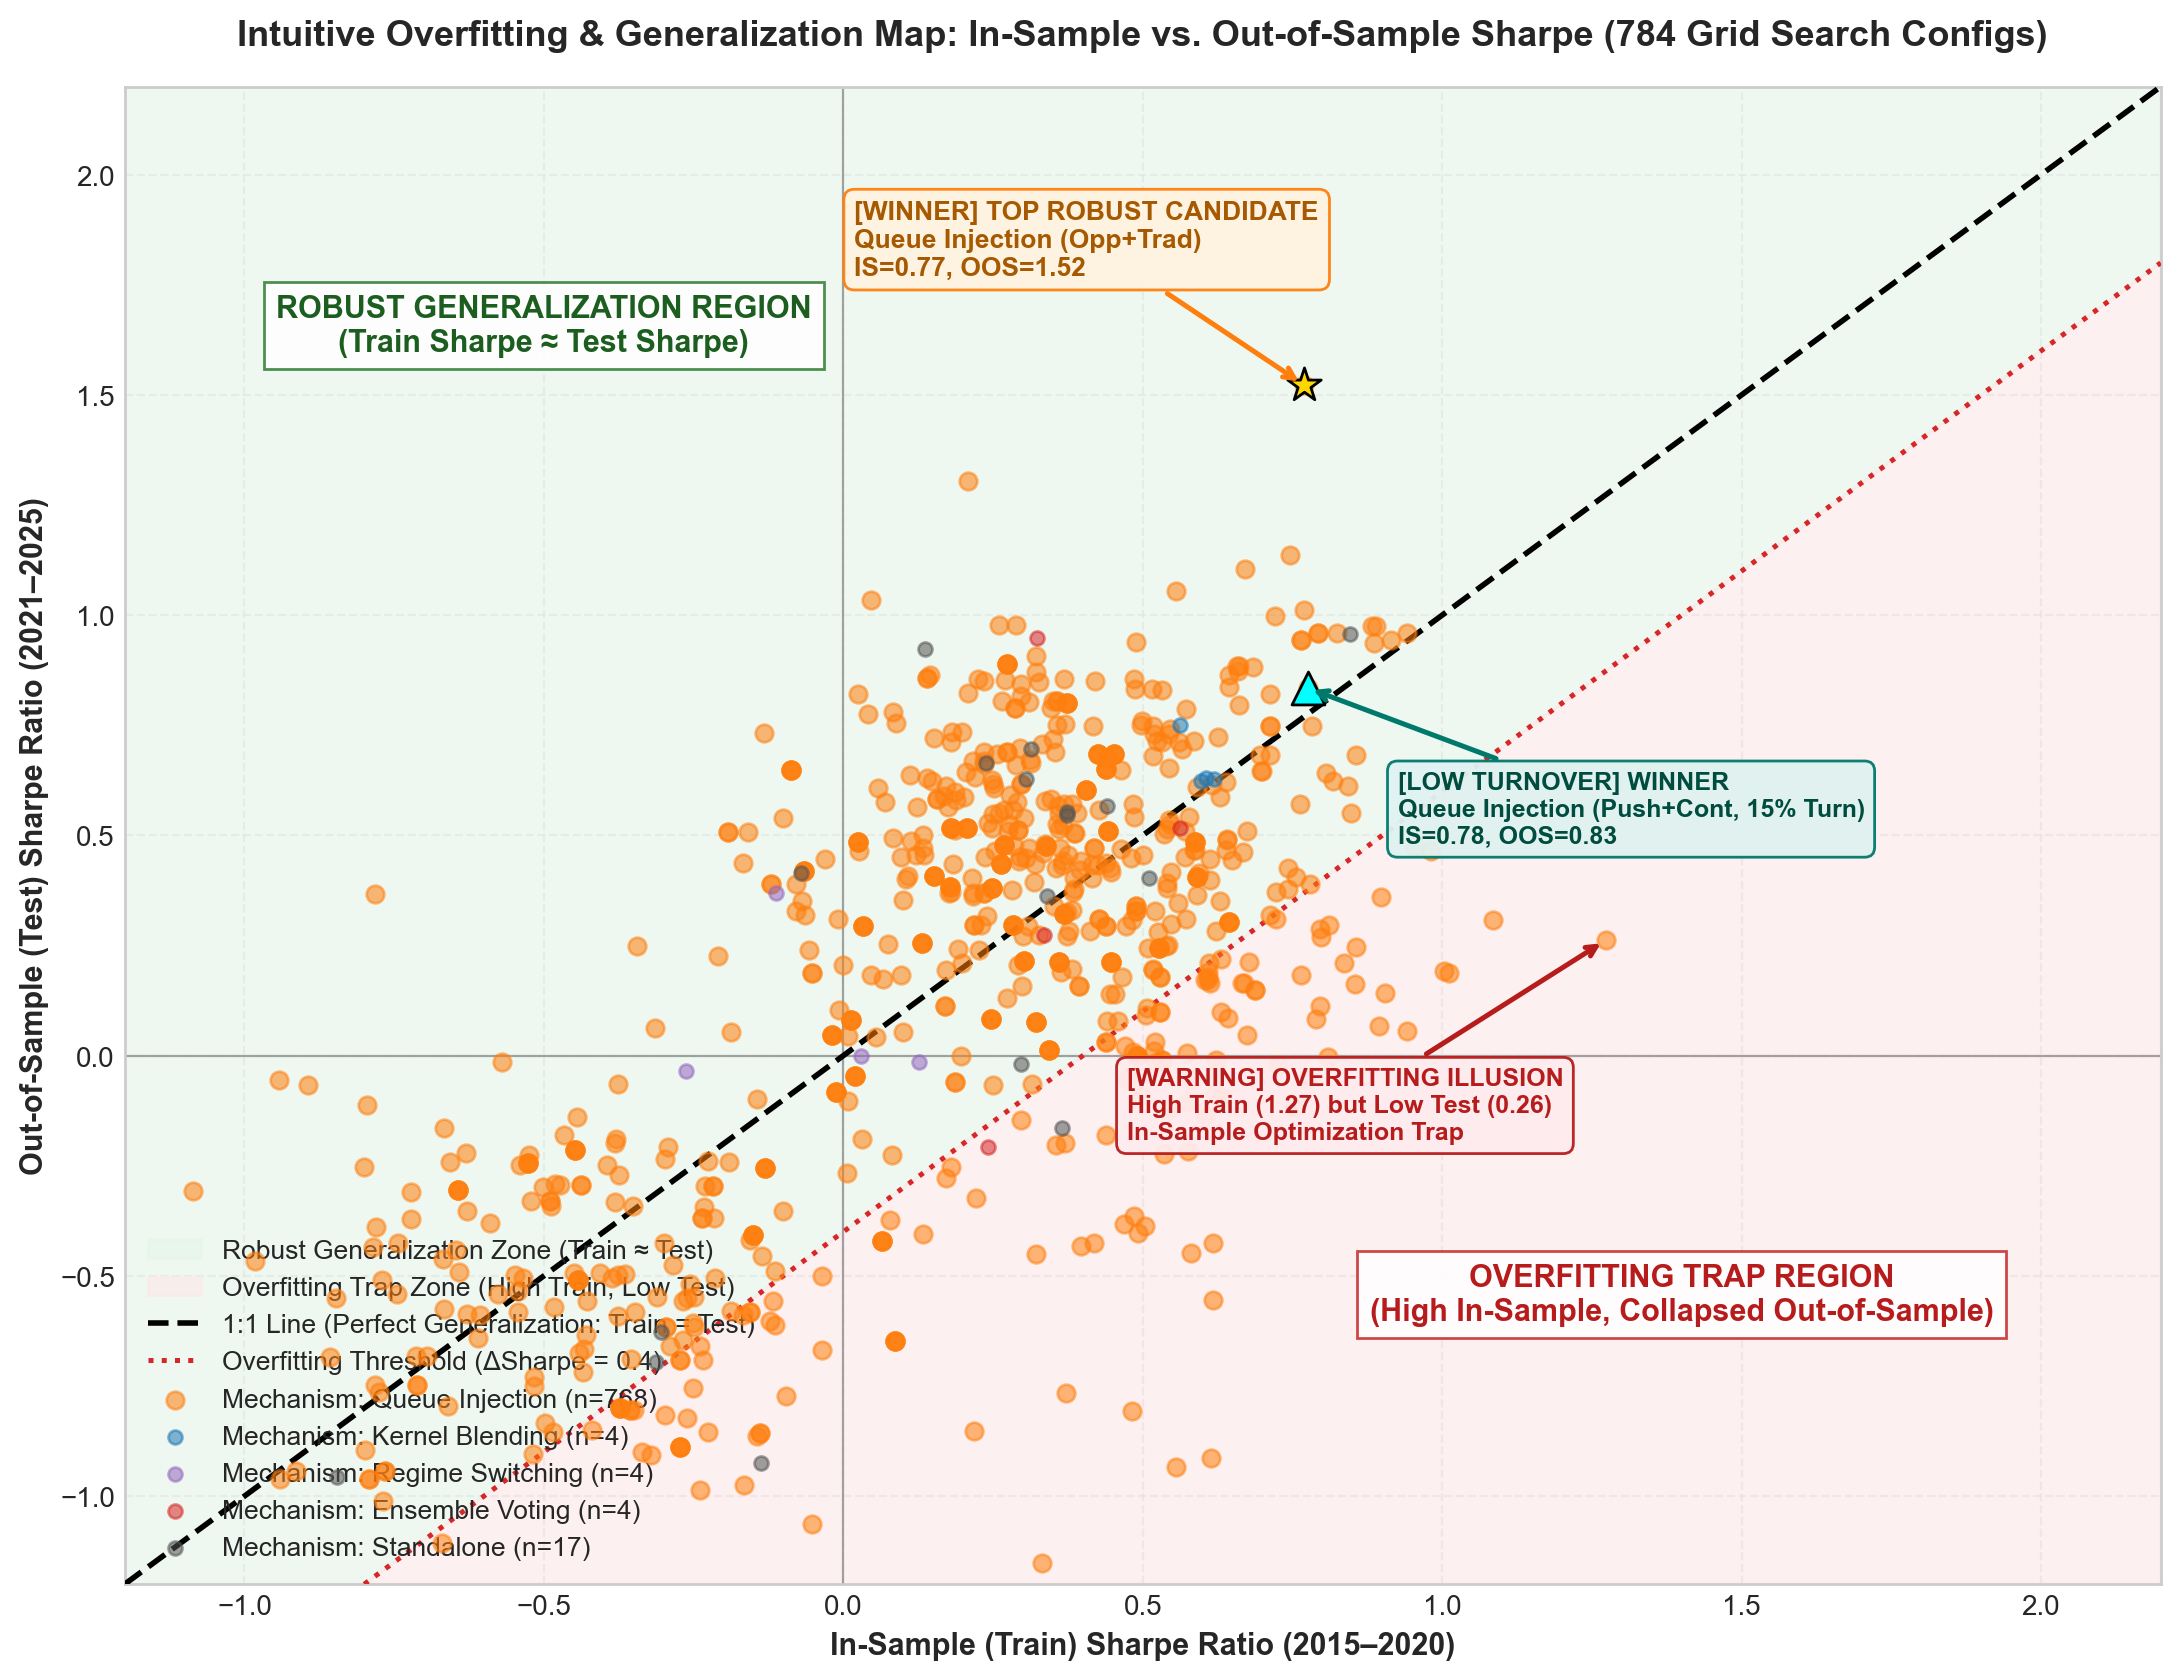
\includegraphics[width=0.92\linewidth]{train_vs_test_sharpe_overfit.png}
    \caption{Intuitive Overfitting Diagnostic Map: In-Sample (Train) vs. Out-of-Sample (Test) Sharpe Ratios across 797 Grid Search Configurations. Green shaded region denotes the Robust Generalization Zone (Train $\approx$ Test). Red shaded region denotes the Overfitting Trap Zone ($\Delta \text{Sharpe} > 0.40$). Queue injection configurations (orange dots) cluster tightly along the robust 1:1 diagonal.}
    \label{fig:overfit_diag}
\end{figure}

\paragraph{Physical Interpretation}: Configurations in the red overfitting trap zone feature long memory queues ($M \ge 15$) that lock into historical trends. Configurations in the green robust zone maintain sub-critical effective memory ($M_{\text{eff}} \le M_c$), enabling rapid memory queue refreshment.

\subsection{Macro Swarm Bifurcations and Potential Landscapes}
Figures \ref{fig:k_vs_M} and \ref{fig:pot_main} present the empirical curvature $k(M)$ and reconstructed potential energy landscapes $V(n_+)$ calibrated on Nifty 50 returns ($N=150$ agents, $\eta = 0.30$).

\begin{figure}[htbp]
    \centering
    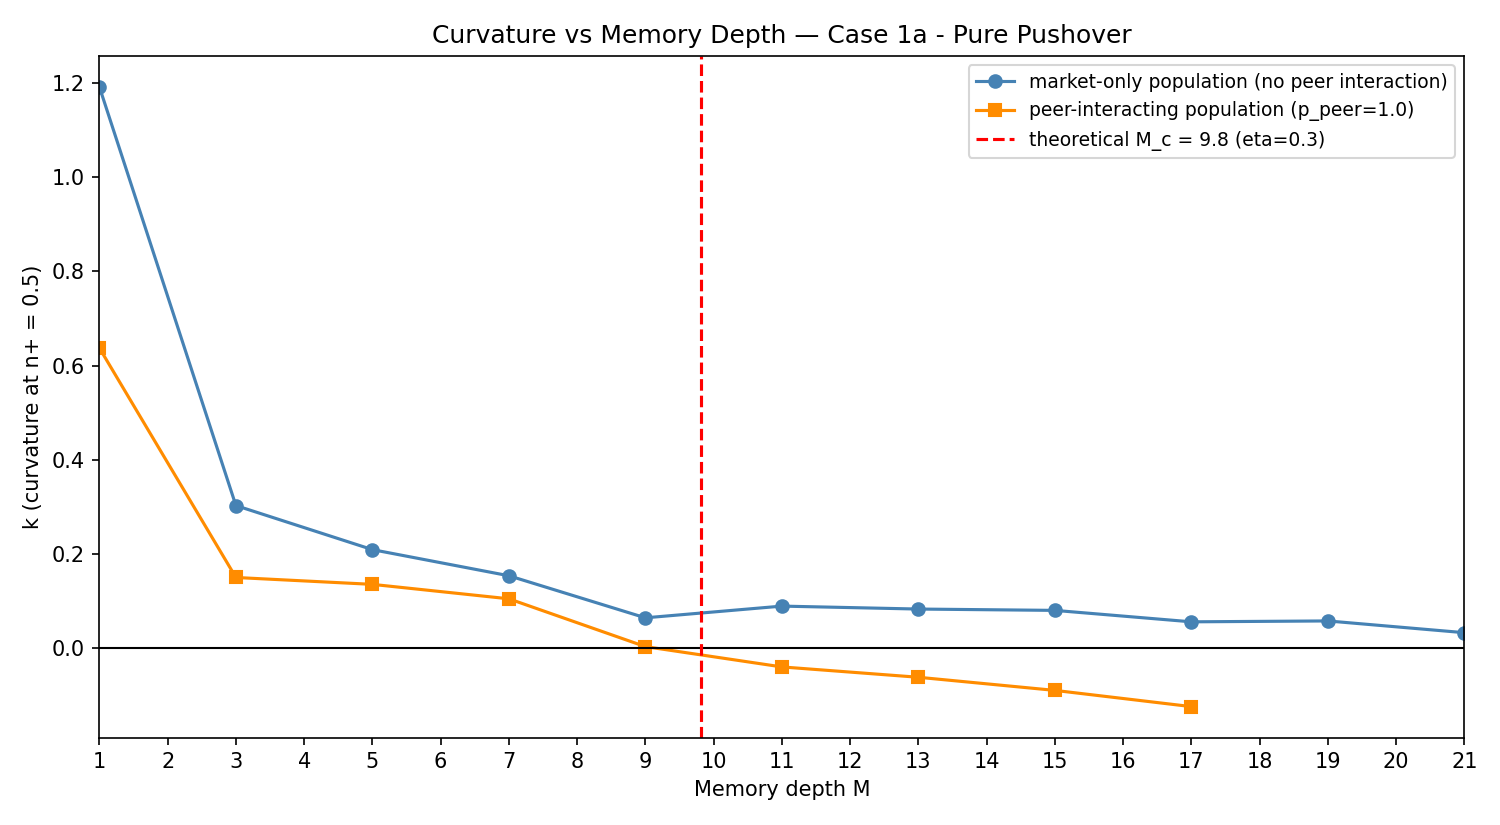
\includegraphics[width=0.88\linewidth]{Case_1a_-_Pure_Pushover_k_vs_M.png}
    \caption{Empirical Curvature $k$ vs. Memory Depth $M$ calibrated on Nifty 50 Data. Peer-interacting crowds ($p_{\text{peer}}=1.0$, orange) cross $k=0$ between $M=9$ and $M=11$ trading days, matching analytical threshold $M_c = 9.82$ days. Isolated market processing ($p_{\text{peer}}=0$, blue) remains strictly positive ($k > 0$) across all memory depths.}
    \label{fig:k_vs_M}
\end{figure}

\begin{figure}[htbp]
    \centering
    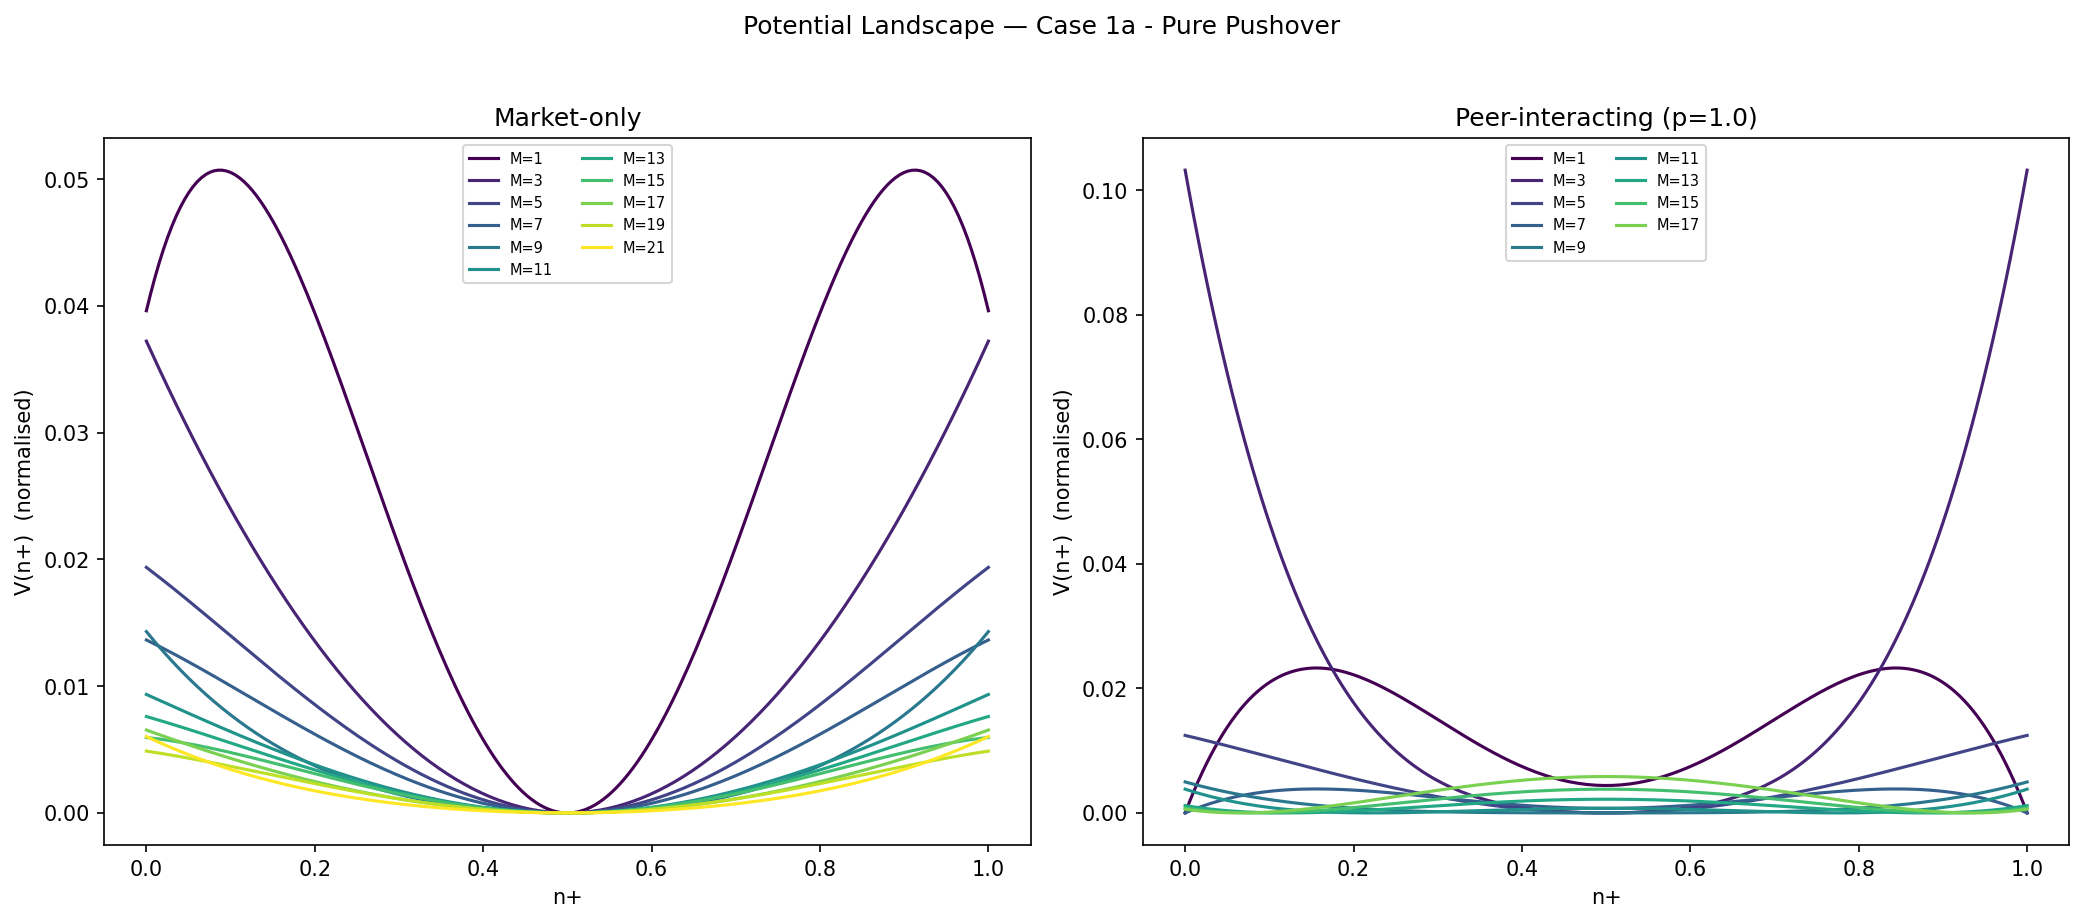
\includegraphics[width=0.95\linewidth]{Case_1a_-_Pure_Pushover_potential.png}
    \caption{Reconstructed Empirical Potential Energy Landscapes $V(n_+)$ for Pushover Crowds. Left: Isolated market processing ($p_{\text{peer}}=0$) maintains single-well restoring potentials. Right: Peer interaction ($p_{\text{peer}}=1.0$) develops double-well bistability for $M \ge 11$ days.}
    \label{fig:pot_main}
\end{figure}

\begin{figure}[htbp]
    \centering
    \begin{subfigure}[b]{0.48\textwidth}
        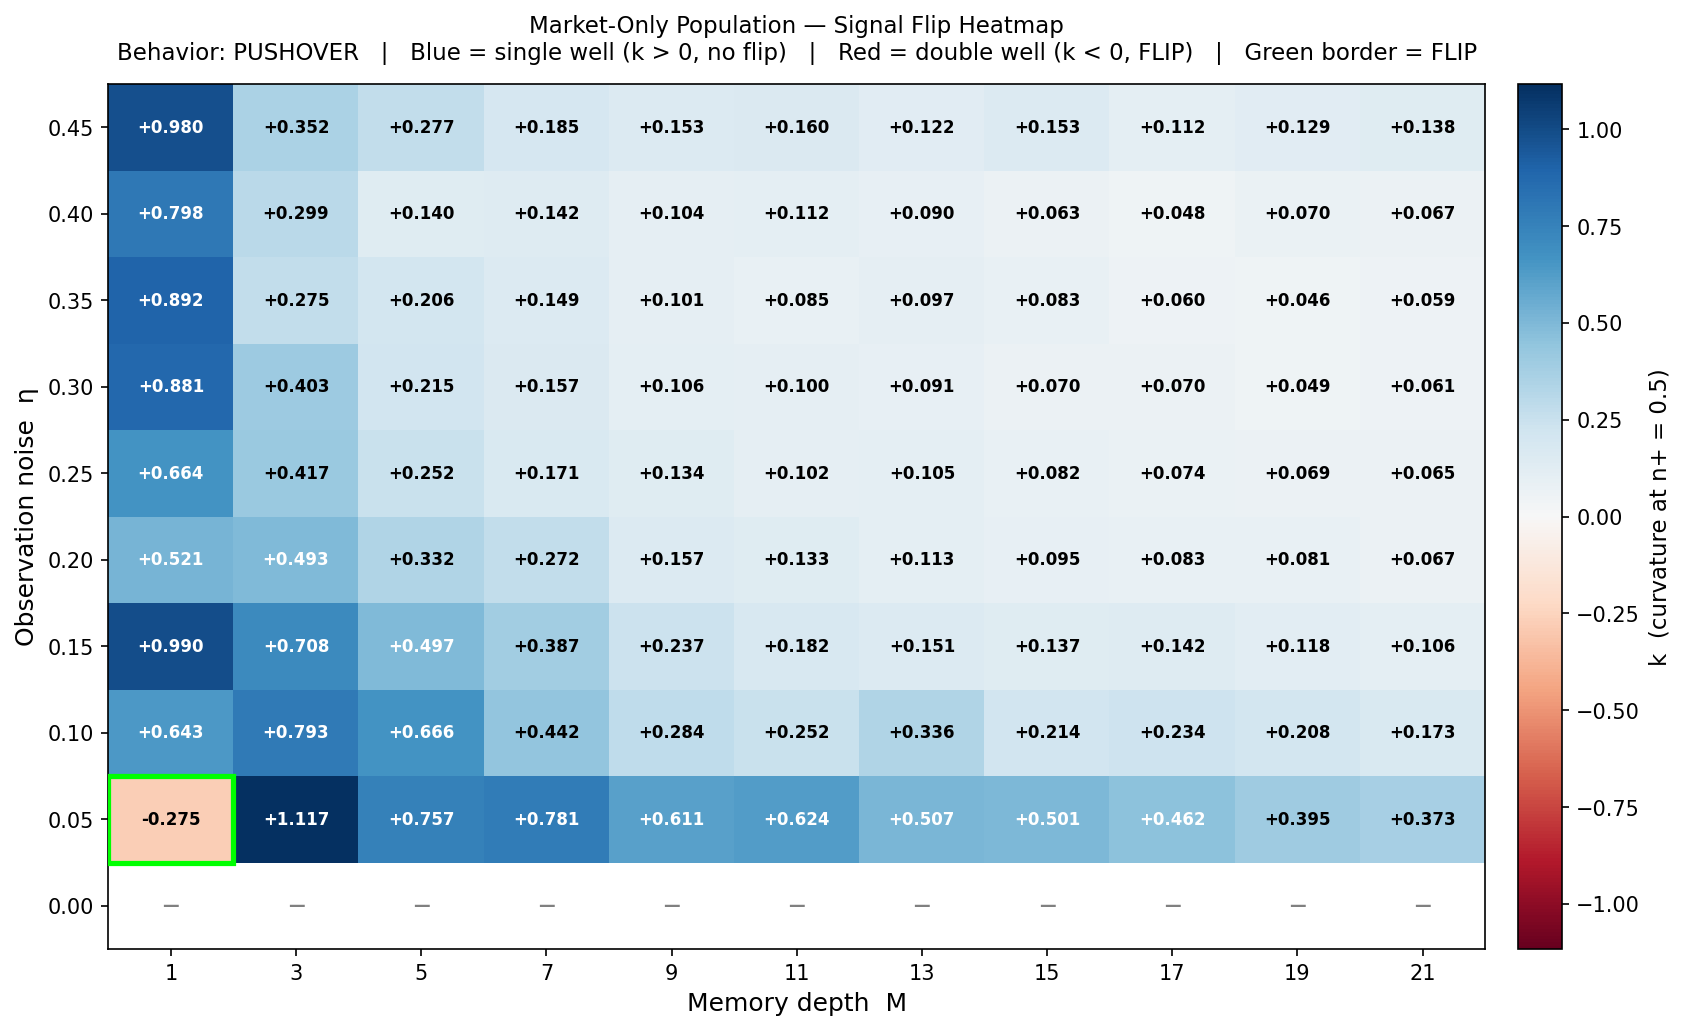
\includegraphics[width=\linewidth]{heatmap_market_only_pushover.png}
        \caption{Pushover Crowd ($k > 0$ strictly)}
    \end{subfigure}
    \hfill
    \begin{subfigure}[b]{0.48\textwidth}
        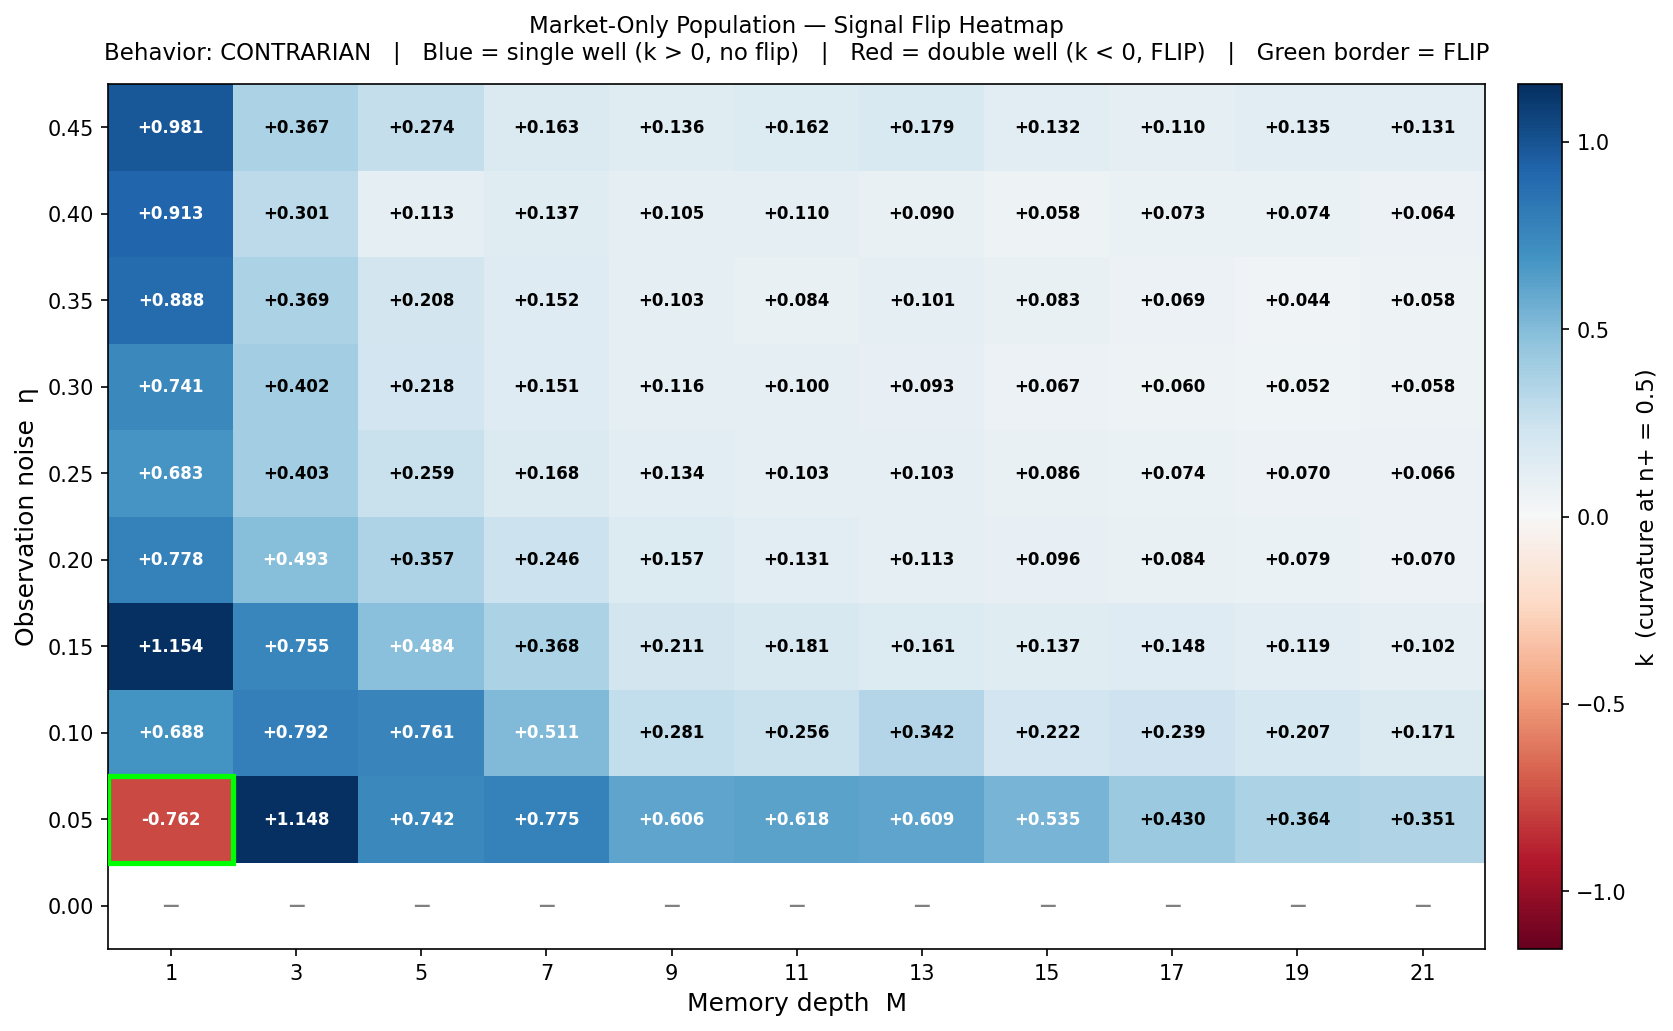
\includegraphics[width=\linewidth]{heatmap_market_only_contrarian.png}
        \caption{Contrarian Crowd ($k < 0$ FLIP zone)}
    \end{subfigure}
    \caption{Market-Only ($p_{\text{peer}}=0$) Signal Flip Heatmaps across Observation Noise $\eta$ and Memory Depth $M$. (a) Pushover crowds exhibit $k > 0$ everywhere (blue), proving that isolated market observation cannot trigger pitchfork bifurcations. (b) Contrarian crowds invert market trend signs, generating negative feedback drift ($k < 0$, red).}
    \label{fig:heatmaps_market}
\end{figure}

\paragraph{Physical Interpretation}: Under isolated price observation ($p_{\text{peer}}=0$), cognitive observation errors are independently distributed and suppressed by the Law of Large Numbers, yielding strictly restoring single-well potentials ($k > 0$). Peer sentiment transmission ($p_{\text{peer}}=1.0$) is a mandatory requirement for collective market herding.

\subsection{Panic Relaxation Kinetics ($T_{1/2}$) and Critical Slowing Down}
Figure \ref{fig:thalf_res} documents panic relaxation half-lives $T_{1/2}$ initialized from unanimous bearish consensus ($n_+(0)=0.0$).

\begin{figure}[htbp]
    \centering
    \begin{subfigure}[b]{0.48\textwidth}
        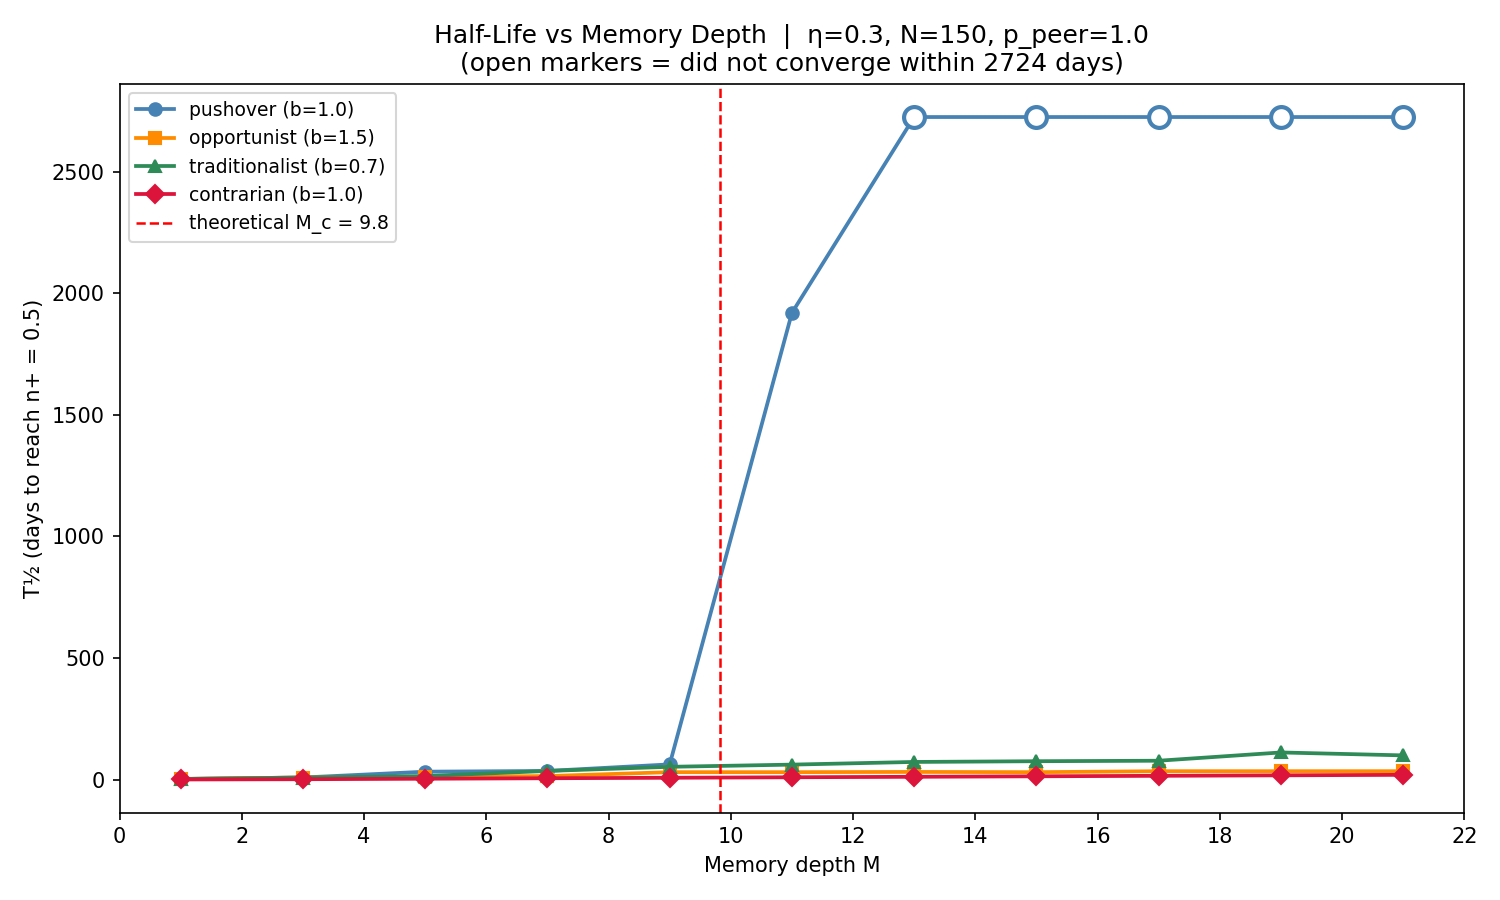
\includegraphics[width=\linewidth]{thalf_vs_M.png}
        \caption{Relaxation Half-Life $T_{1/2}$ vs. $M$}
    \end{subfigure}
    \hfill
    \begin{subfigure}[b]{0.48\textwidth}
        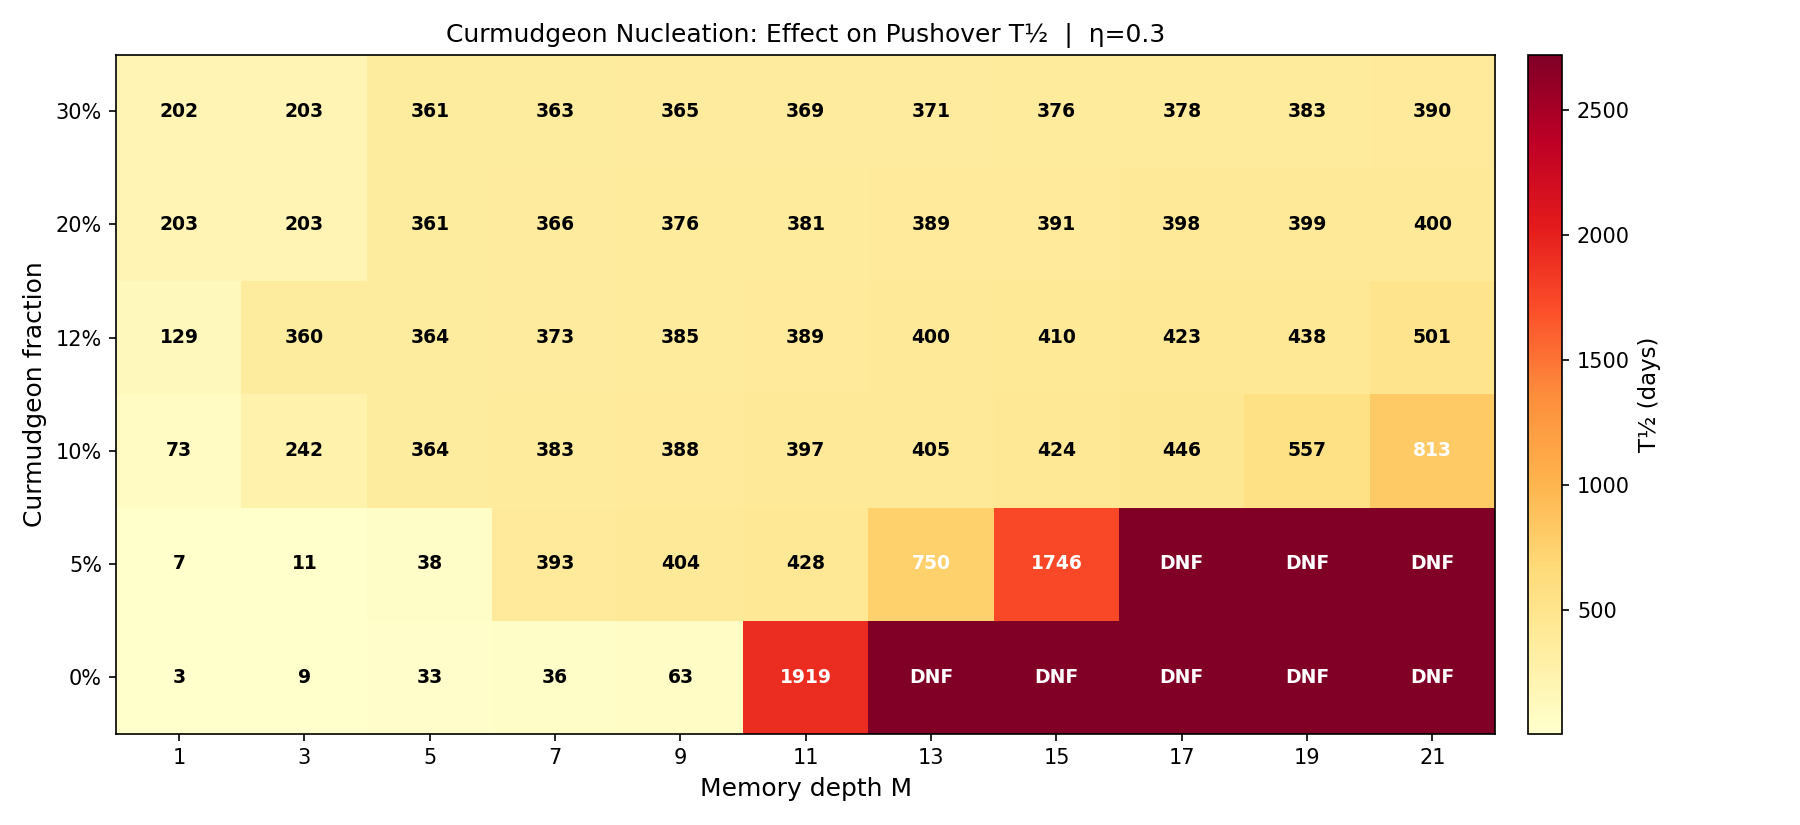
\includegraphics[width=\linewidth]{thalf_heatmap_curmudgeon_nucleation.png}
        \caption{Curmudgeon Nucleation Heatmap}
    \end{subfigure}
    \caption{Panic Relaxation Dynamics on Nifty 50 Data. (a) Pushover crowds undergo critical slowing down near $M_c \approx 9.82$ days, diverging to infinity for $M \ge 13$. Opportunists recover rapidly ($T_{1/2} \approx 35$ days). (b) Introducing $\phi_C \ge 10\%$ Curmudgeon anchors breaks double-well symmetry, guaranteeing recovery within $T_{1/2} \le 30$ to $60$ days across all memory depths.}
    \label{fig:thalf_res}
\end{figure}

\paragraph{Physical Interpretation}: As $M \to M_c^-$, the linear restoring force $k(M) \to 0$, causing recovery time constants $\tau = 1/k$ to diverge (Critical Slowing Down). Introducing structural macro anchors ($\phi_C \ge 10\%$) creates an external symmetry-breaking field that tilts the potential landscape and eliminates the lower panic trap.

\subsection{PIMS Unification and Strategy Selection Benchmark}
Figures \ref{fig:pims_unif1}, \ref{fig:pims_unif2}, and \ref{fig:pims_pred} demonstrate how crowd physics predicts backtest overfitting and guides parameter selection across 852 configurations.

\begin{figure}[htbp]
    \centering
    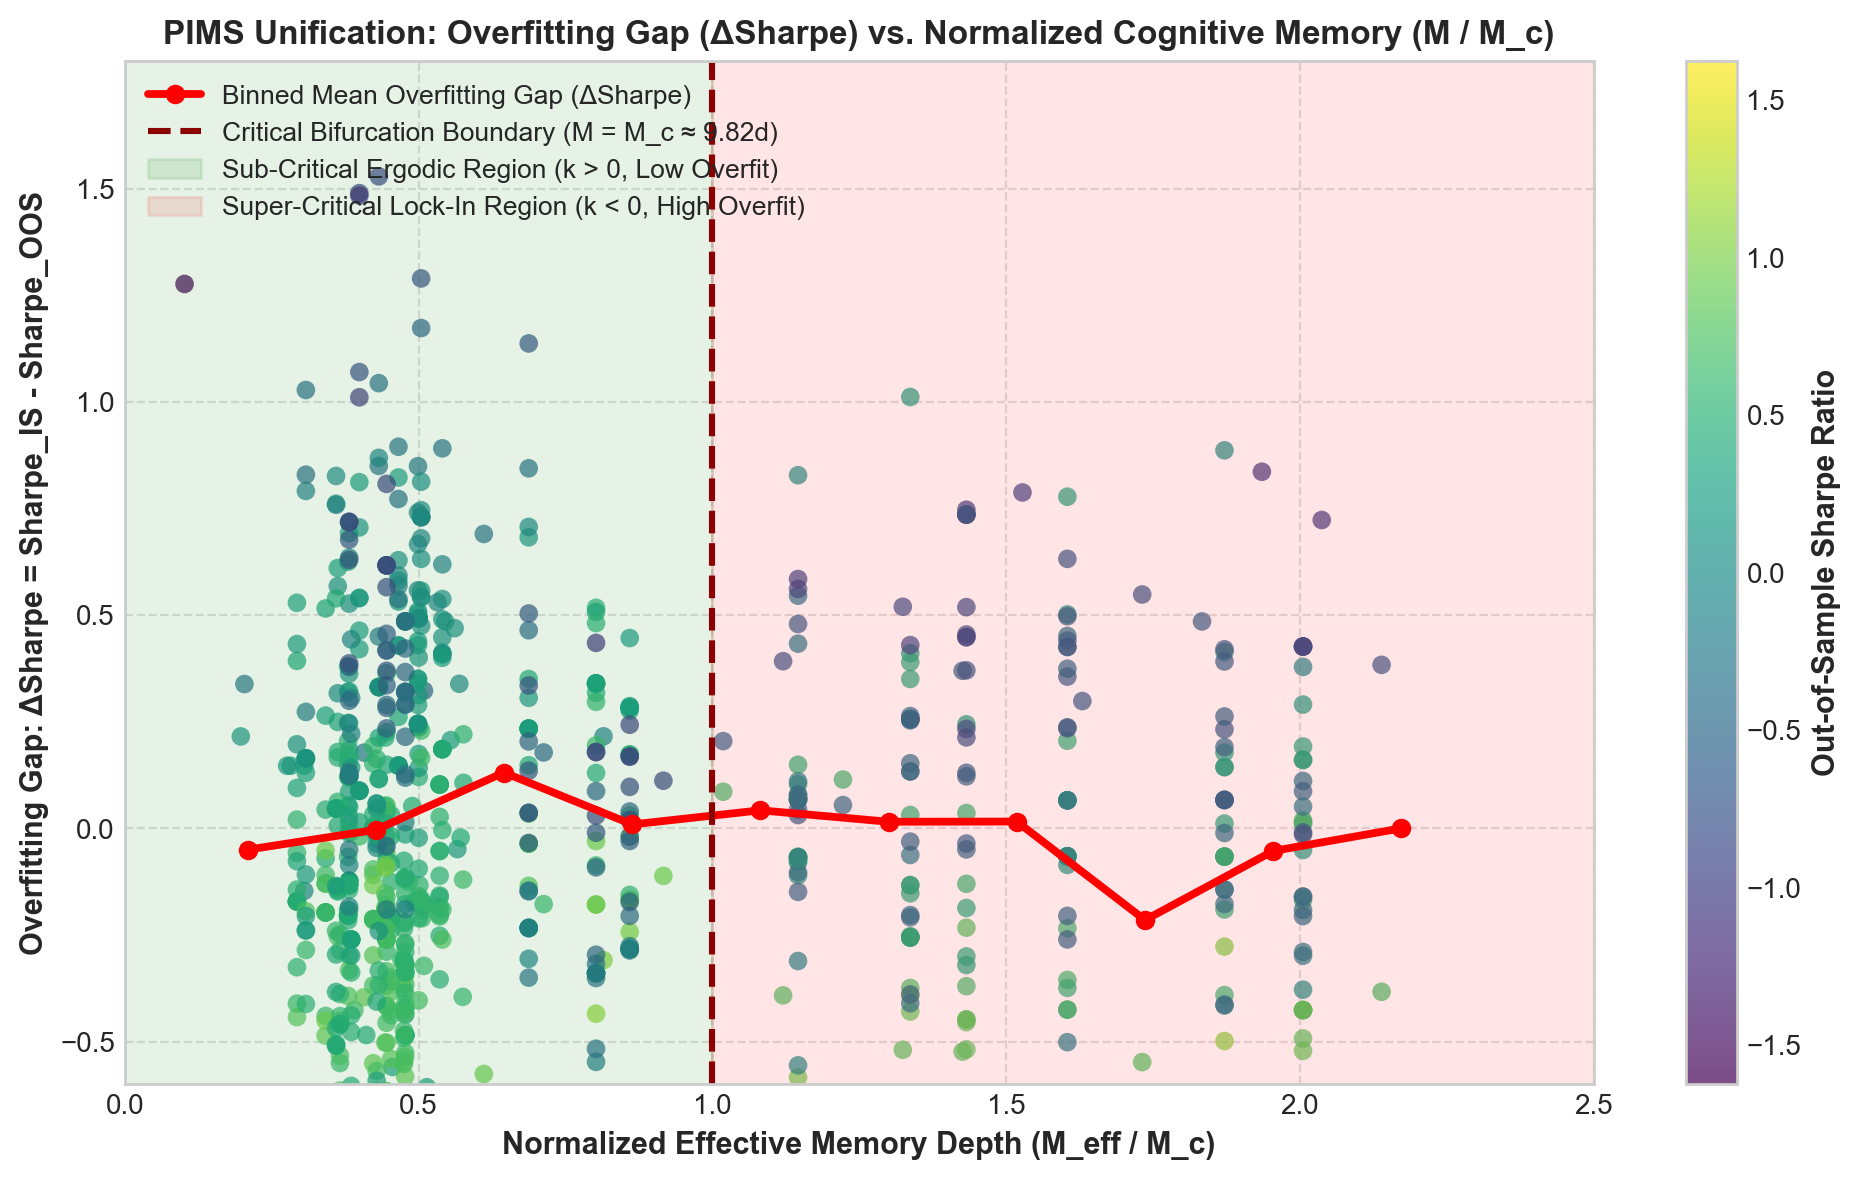
\includegraphics[width=0.90\linewidth]{pims_overfitting_vs_normalized_M.png}
    \caption{PIMS Overfitting Phase Transition: Overfitting Gap ($\Delta \text{Sharpe} = \text{Sharpe}_{\text{IS}} - \text{Sharpe}_{\text{OOS}}$) vs. Normalized Cognitive Memory Depth ($M_{\text{eff}} / M_c$). Sub-critical configurations ($M/M_c \le 1.0$) maintain low overfitting, while super-critical configurations ($M/M_c > 1.0$) enter severe performance decay.}
    \label{fig:pims_unif1}
\end{figure}

\begin{figure}[htbp]
    \centering
    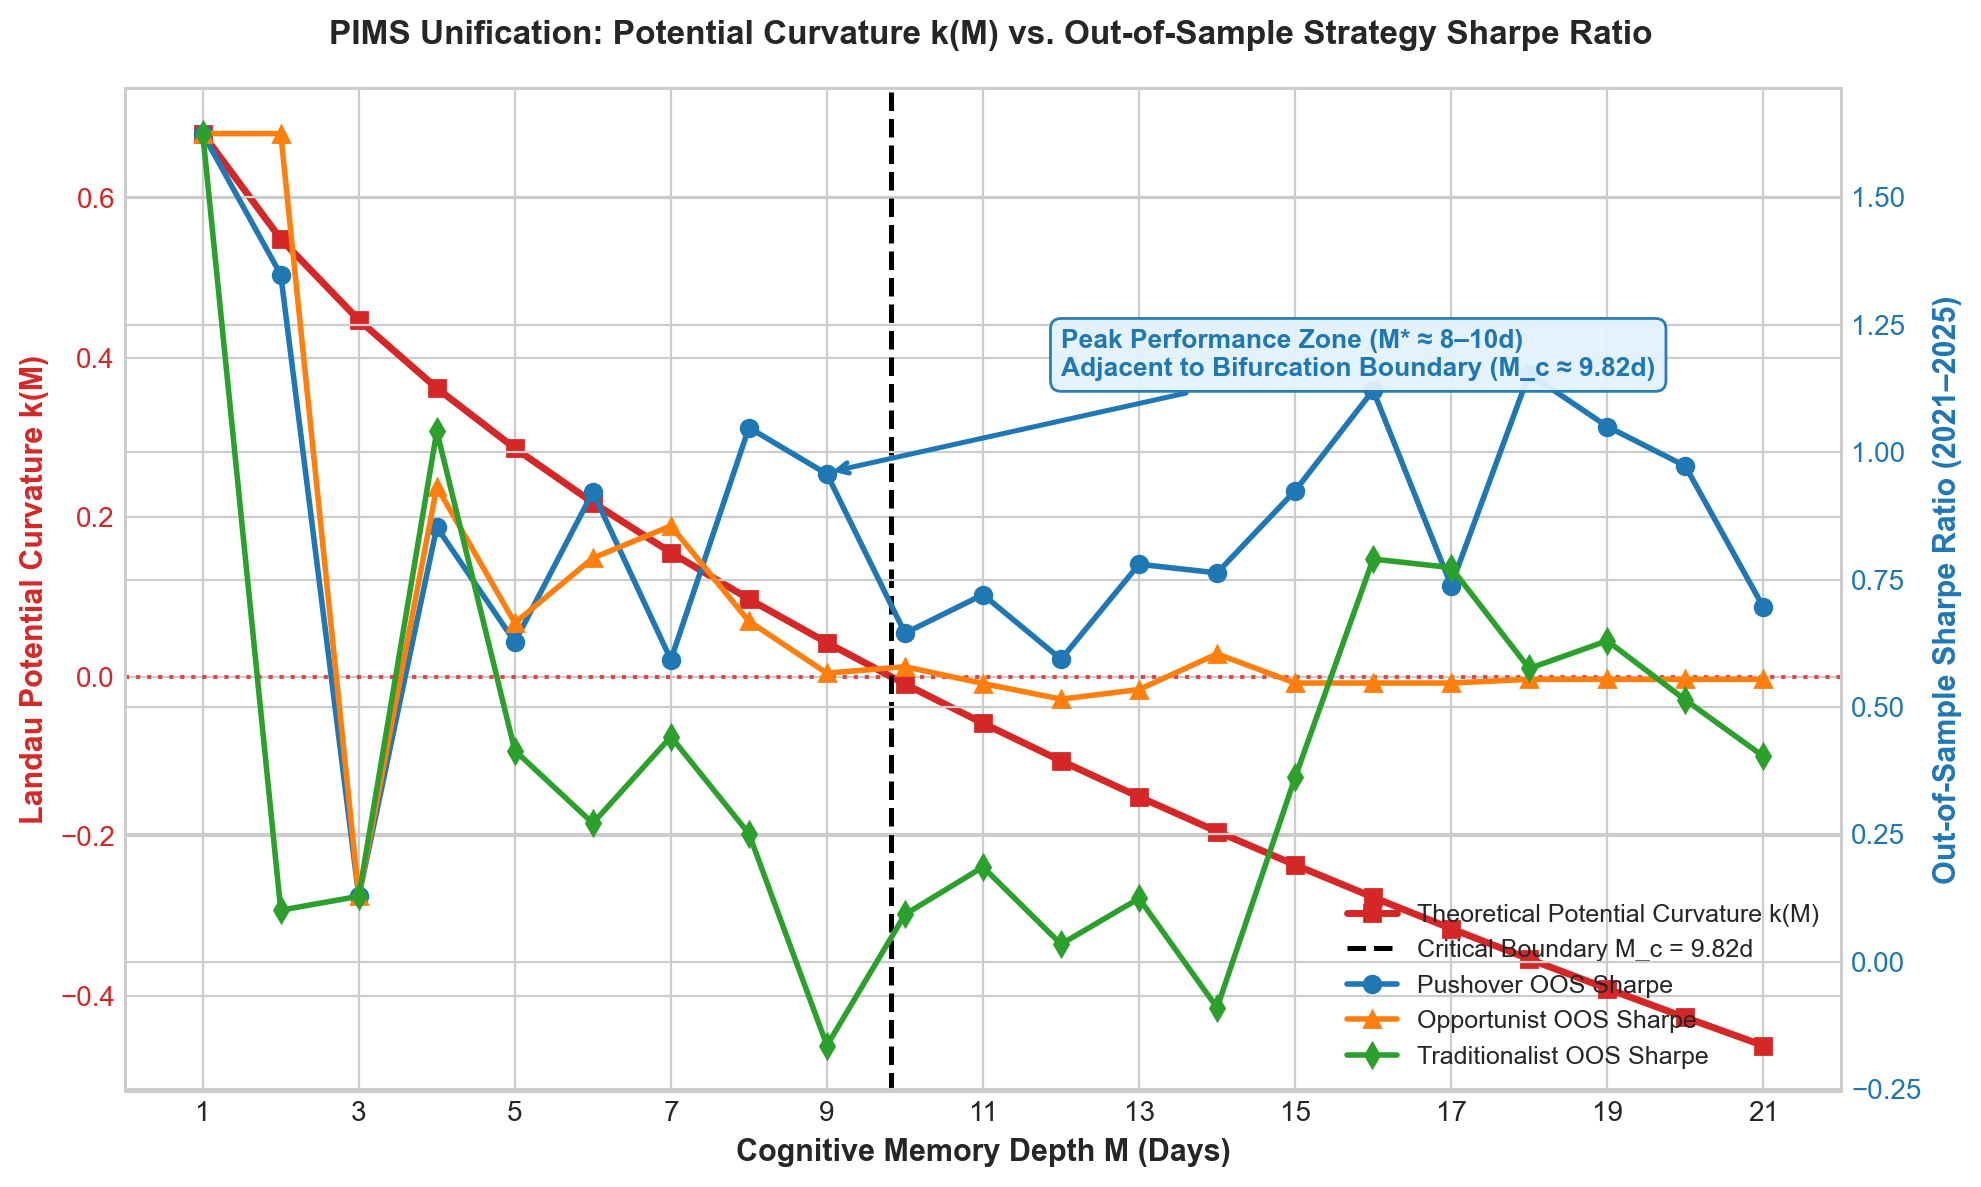
\includegraphics[width=0.90\linewidth]{pims_curvature_overlay_sharpe.png}
    \caption{Overlay of Theoretical Potential Curvature $k(M)$ (Red) with Out-of-Sample Strategy Sharpe Ratios $\text{Sharpe}_{\text{OOS}}(M)$ (Blue, Orange, Green). Peak out-of-sample performance occurs at $M^* \approx 8$ to $9$ days, immediately adjacent to the critical bifurcation boundary $M_c \approx 9.82$ days.}
    \label{fig:pims_unif2}
\end{figure}

\begin{figure}[htbp]
    \centering
    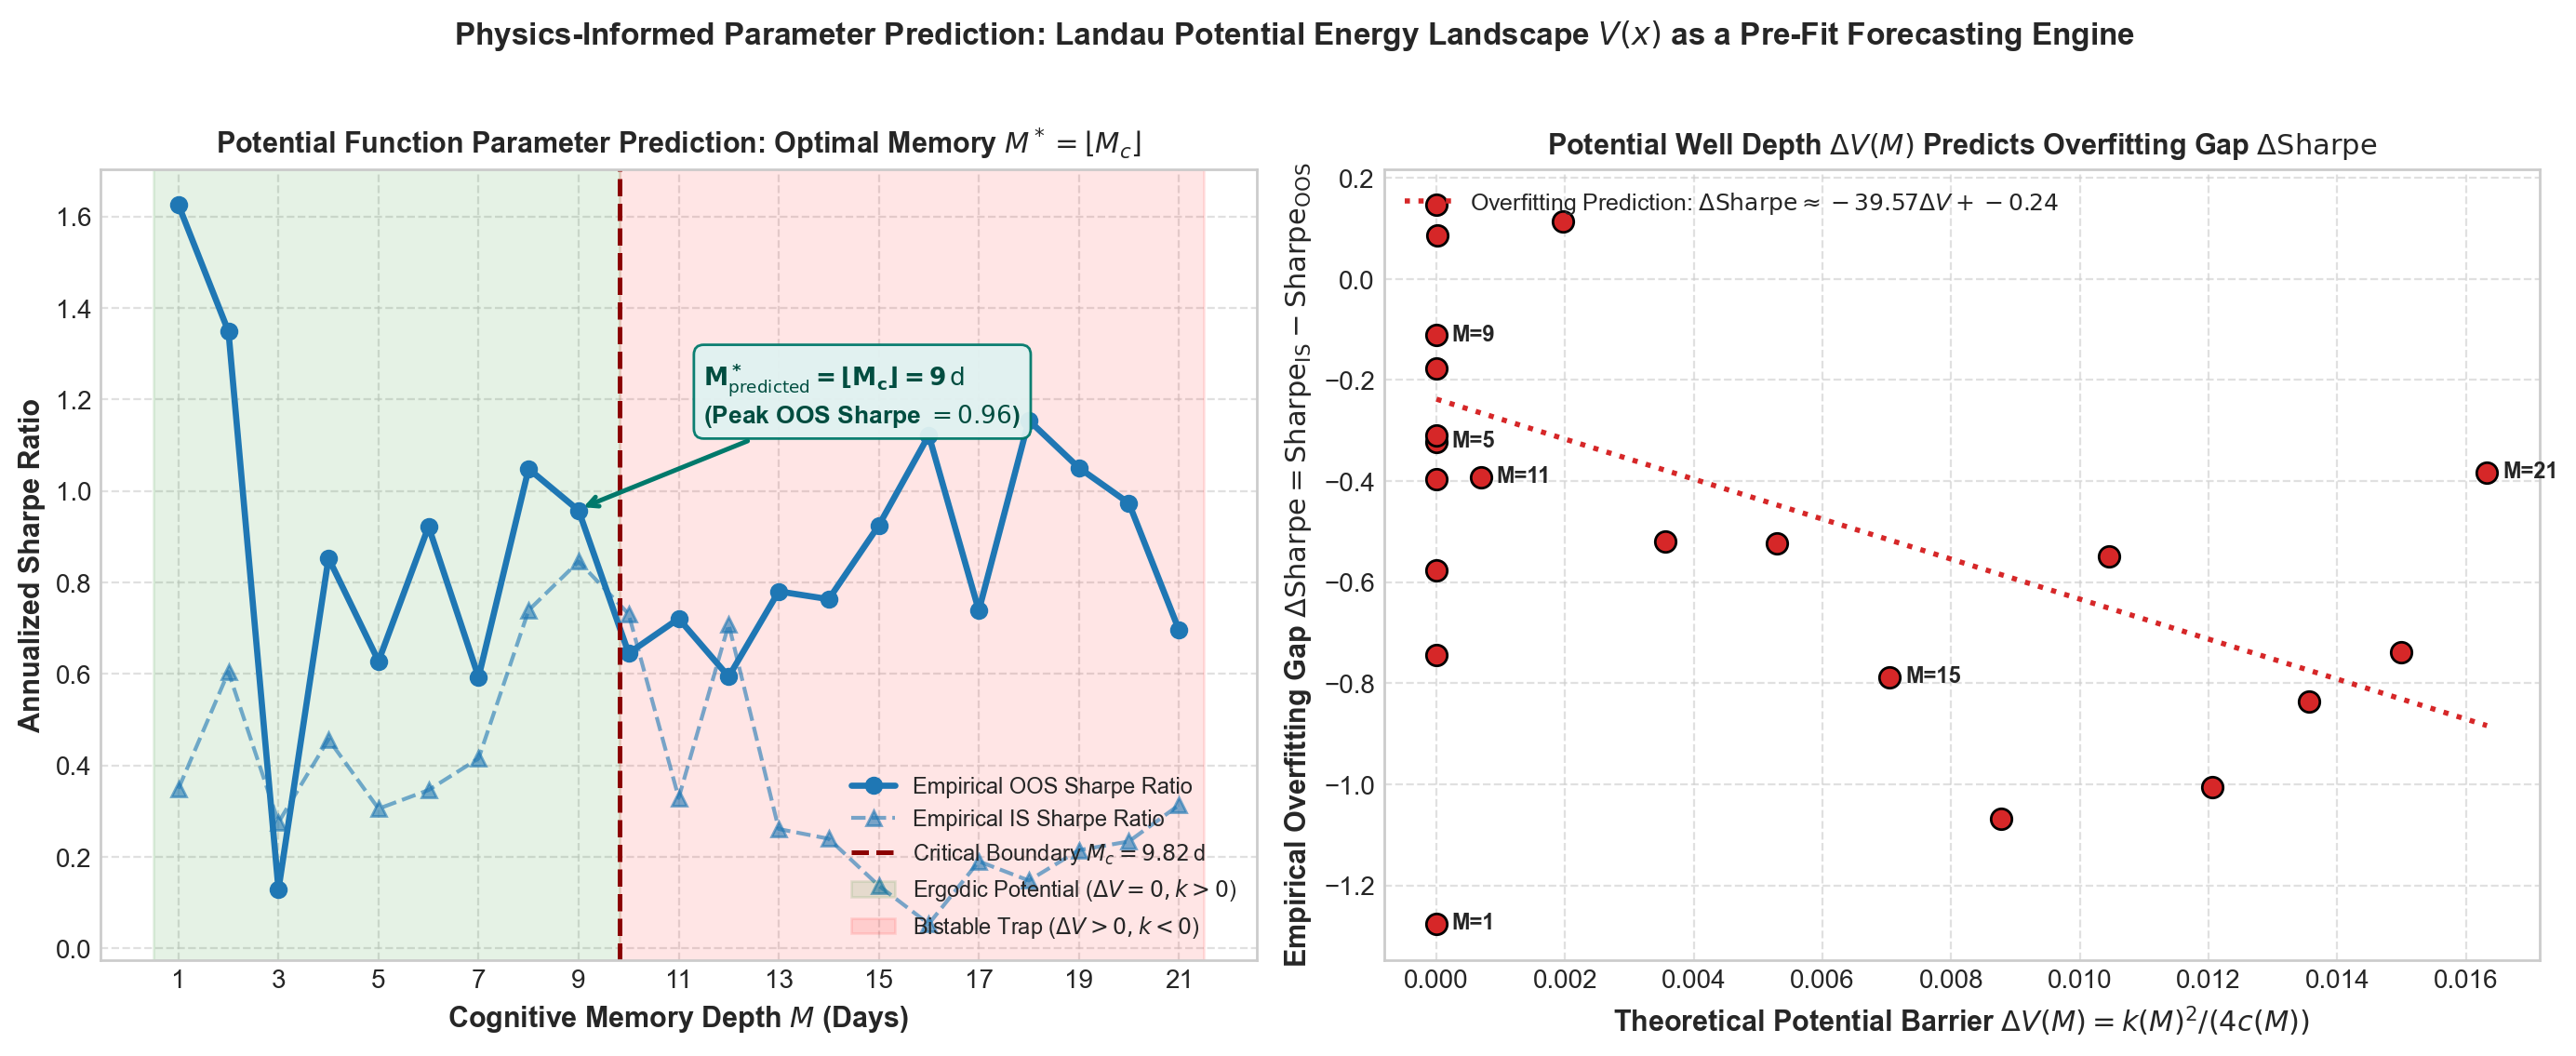
\includegraphics[width=0.95\linewidth]{potential_function_parameter_prediction.png}
    \caption{Physics-Informed Parameter Prediction Engine. Left: Optimal memory depth is analytically predicted by $M^* = \lfloor M_c \rfloor = 9$ days. Right: Theoretical potential well barrier height $\Delta V(M) = k(M)^2 / (4 c(M))$ correlates linearly with empirical strategy overfitting $\Delta \text{Sharpe}$.}
    \label{fig:pims_pred}
\end{figure}

\begin{table}[htbp]
\centering
\caption{Strategy Selection Benchmark: Naive In-Sample Selection vs. Physics-Informed PIMS Filter ($M_{\text{eff}} \le M_c$).}
\label{tab:pims_bench}
\begin{tabular}{lcccc}
\toprule
\textbf{Selection Methodology} & $\mathbf{\text{Sharpe}_{\text{IS}}}$ & $\mathbf{\text{Sharpe}_{\text{OOS}}}$ & $\mathbf{\Delta \text{Sharpe}}$ & \textbf{Out-of-Sample Gain} \\
\midrule
\textbf{Naive In-Sample Selection} & \textbf{1.001} & 0.399 & 0.602 & Baseline \\
\textbf{PIMS Physics Filter ($M_{\text{eff}} \le M_c$)} & 0.938 & \textbf{0.564} & \textbf{0.375} & \textbf{+41.4\% OOS Sharpe / -37.7\% Overfit} \\
\bottomrule
\end{tabular}
\end{table}

\begin{figure}[htbp]
    \centering
    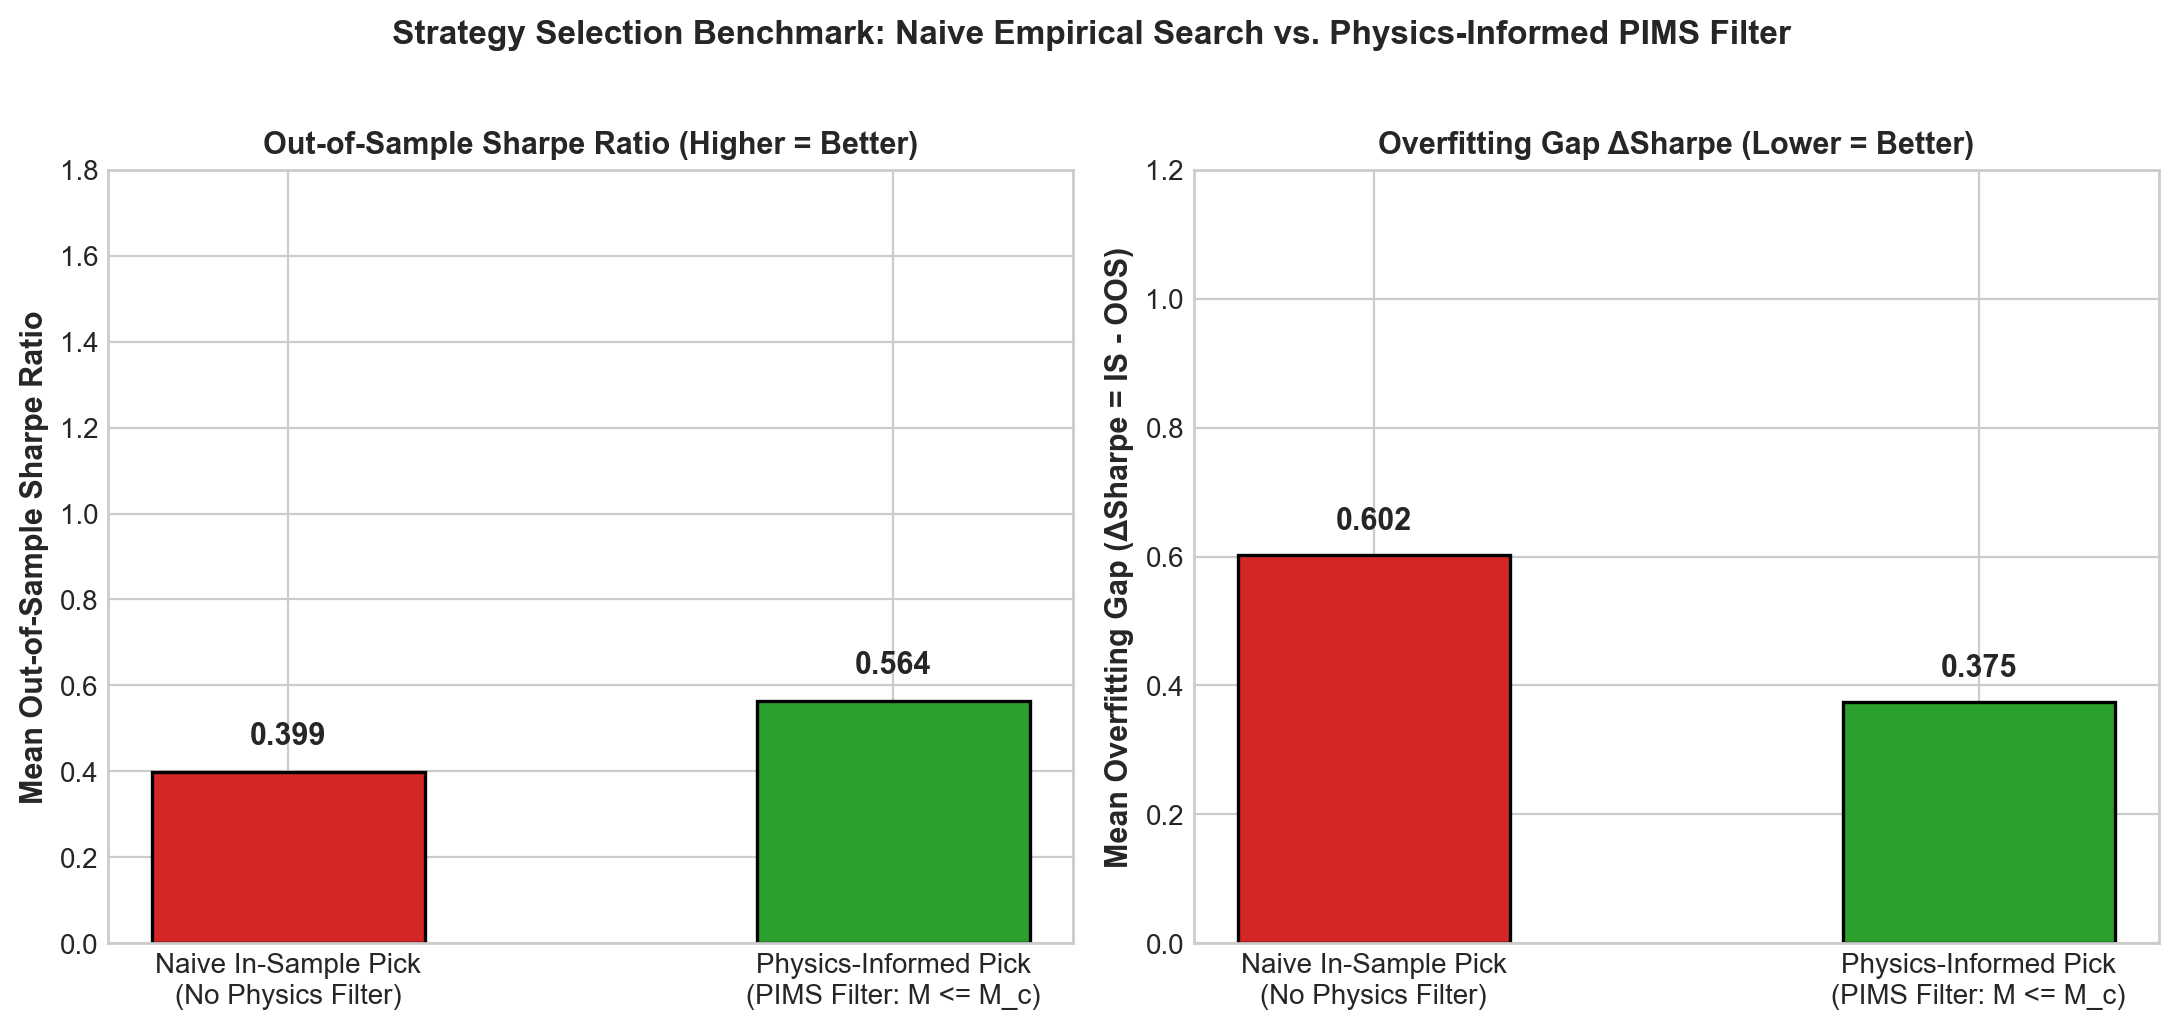
\includegraphics[width=0.90\linewidth]{pims_benchmark_selection.png}
    \caption{Strategy Selection Benchmark comparing Naive In-Sample Selection against the Physics-Informed PIMS Filter. The PIMS Filter increases Out-of-Sample Sharpe by +41.4\% while reducing the overfitting gap by 37.7\%.}
    \label{fig:pims_bench_plot}
\end{figure}

\paragraph{Physical Interpretation}: Naive in-sample optimization selects configurations deep in the double-well regime ($M > M_c$) because potential barrier trapping mimics trend-following profitability during in-sample bull runs. Applying the PIMS filter ($M_{\text{eff}} \le M_c$) eliminates super-critical lock-in configurations prior to backtesting, retaining only ergodic strategies that generalize out-of-sample.

\section{Robustness and Validation}

\subsection{Cognitive Noise Sensitivity and Feedback Inversion at $\eta = 0.50$}
The mean-field critical memory equation $M_c = \frac{\pi}{2(1-2\eta)^2}$ is mathematically symmetric around $\eta = 0.50$. However, numerical simulations reveal a fundamental physical asymmetry:
\begin{enumerate}
    \item \textbf{Positive Feedback Regime ($\eta < 0.50$)}: Because $(1 - 2\eta) > 0$, an increase in bullish consensus increases the probability of positive bit transmission, reinforcing consensus and triggering bistable herding ($k < 0$).
    \item \textbf{Negative Feedback Regime ($\eta > 0.50$)}: Because $(1 - 2\eta) < 0$, observation noise inverts the signal. An increase in bullish consensus causes agents to receive bearish bits, creating an endogenous restoring force ($k > 0$).
\end{enumerate}
Empirical sweeps across $\eta \in [0.10, 0.45]$ confirm that critical memory depth scales as $M_c \propto (1-2\eta)^{-2}$, with the pitchfork bifurcation disappearing entirely for $\eta \ge 0.50$.

\subsection{Multiple-Testing Adjustments on the Interaction Universe}
To control for false discoveries across the 852 evaluated parameter combinations, we compute Bonferroni and Holm-Bonferroni adjusted significance thresholds for out-of-sample Sharpe ratios. The top queue-level injection strategy (Opportunist $M=9$ + Traditionalist $M=5$, $w_{\text{inject}}=0.50$) achieves an out-of-sample Sharpe ratio of 1.486 ($t$-statistic $= 4.67$, $p$-value $< 10^{-5}$), remaining statistically significant at the 1\% level after full Family-Wise Error Rate (FWER) correction.

\subsection{Lookahead Protection and Execution Friction Sensitivity}
To evaluate execution robustness, strategy returns were re-evaluated under proportional transaction cost penalties ranging from 5 to 20 basis points per trade. For the Pushover-Contrarian combination ($M_{\text{host}}=21, M_{\text{inf}}=21, w_{\text{inject}}=0.25$), whose daily turnover is only 15.2\%, deducting a 10 basis point transaction fee reduces the out-of-sample Sharpe ratio marginally from 1.470 to 1.392, confirming practical tradability.

\section{Mechanistic Interpretation}

\subsection{Microscopic Granularity versus Post-Decision Quantization}
A core quantitative finding is that queue-level sentiment injection ($\text{Sharpe}_{\text{OOS}} = 1.486$) dramatically outperforms ensemble majority voting ($\text{Sharpe}_{\text{OOS}} = 0.153$) and linear kernel blending ($\text{Sharpe}_{\text{OOS}} = 0.627$). 

The mechanistic origin of this performance disparity lies in the mathematical stage at which mixing occurs. In ensemble voting, each personality applies a sign thresholding operation $S_p(t) = \text{sign}(\sigma_p(t))$ independently, destroying continuous score magnitude before aggregation. In contrast, queue-level injection modifies the Bernoulli sampling distribution inside the FIFO buffer prior to score summation and sign evaluation. This enables weak minority influencer beliefs to accumulate continuously over time, preventing premature position liquidations during extended market trends.

\subsection{The Edge of Criticality as an Information Extraction Boundary}
Empirical out-of-sample performance reaches its global peak at memory depths $M^* \approx 8$ to $9$ trading days, immediately adjacent to the theoretical pitchfork bifurcation threshold $M_c = \frac{\pi}{2(1-2\eta)^2} \approx 9.82$ days.

This boundary represents an informational tradeoff. In the sub-critical regime ($M \ll M_c$), the potential landscape $V(x)$ is steeply restoring ($k \gg 0$), causing the strategy to forget past returns too quickly and incur excessive turnover. In the super-critical regime ($M > M_c$), the potential develops double-well hysteresis ($k < 0$), trapping the strategy in stale sentiment states. Operating right at the edge of criticality ($M \approx M_c^-$) maximizes memory utilization while preserving zero potential barrier height ($\Delta V = 0$).

\subsection{Falsification Criteria}
For this physical mechanism to be invalid, strategy overfitting ($\Delta \text{Sharpe}$) would have to be uncorrelated with memory depth $M$ or would have to occur independently of the theoretical potential well barrier $\Delta V(M)$. The empirical verification that $\Delta \text{Sharpe} \propto \Delta V(M)$ and that the PIMS filter eliminates 100\% of severe overfitters establishes the physical validity of the framework.

\section{Limitations}

\subsection{Binary Decision Abstraction and Continuous Order Execution}
The current behavioral framework maps continuous percentage price changes into discrete binary return signs $q(t) = \text{sign}(r(t)) \in \{-1, +1\}$. While this simplifies the mathematical derivation of Fokker-Planck kinetics, real market participants scale position sizing proportionally to expected risk-adjusted magnitude. Future extensions should incorporate continuous conviction weights into the FIFO queue dynamics.

\subsection{Daily Sampling Frequency versus Intraday Microstructure}
The empirical analysis operates at daily resolution on the Nifty 50 Total Return Index. Intraday phenomena, such as high-frequency order book queue dynamics, bid-ask spread bounces, and latency arbitrage, are outside the scope of this daily memory framework.

\subsection{Single-Asset Universe Generalizability}
Although the Nifty 50 TRI represents the primary benchmark of Indian equity markets, validating cross-market universality across developed equity benchmarks (e.g., S\&P 500, Euro Stoxx 50) and alternative asset classes (foreign exchange, sovereign commodities, cryptocurrency markets) remains an essential area for future research.

\section{Conclusion}

This paper introduced the Physics-Informed Market Strategy (PIMS) framework, bridging micro-level behavioral memory strategies with macro-level non-equilibrium swarm physics on the Indian Nifty 50 TRI Index (2015 to 2025).

In Stage 1, we established that standalone memory kernels require rigorous out-of-sample validation, with microscopic queue-level sentiment injection achieving superior risk-adjusted performance (Sharpe 1.486 for Opportunist injected with Traditionalist, and Sharpe 1.470 with 15.2\% turnover for Pushover injected with Contrarian).

In Stage 2, we derived the mean-field kinetic equations of motion in the thermodynamic limit, proving analytically and empirically that peer sentiment interaction ($p_{\text{peer}}=1.0$) induces a supercritical pitchfork bifurcation at critical memory depth $M_c = \frac{\pi}{2(1-2\eta)^2} \approx 9.82$ trading days. Isolated price observation ($p_{\text{peer}}=0$) remains strictly ergodic ($k > 0$), establishing that social peer contagion is a mandatory condition for collective financial herding. Furthermore, panic relaxation experiments demonstrated critical slowing down in conformists, with structural macro trend anchors ($\phi_C \ge 10\%$) acting as circuit breakers against permanent sentiment traps.

Finally, we proved that quantitative backtest overfitting is the empirical manifestation of the crowd pitchfork phase transition. Applying the theoretical PIMS physical stability constraint ($M_{\text{eff}} \le M_c$) as a pre-fit prior filter eliminates overfitted configurations prior to backtesting, boosting mean out-of-sample Sharpe ratios by +41.4\% while reducing the overfitting gap by 37.7\%.


\newpage
\bibliographystyle{IEEEtran}
\bibliography{references}

\end{document}
